% Dokumentenklasse und Packages
% Die folgenden Zeilen sollen möglichst nicht verändert werden
\documentclass[paper=a4,bibliography=totoc,BCOR=10mm,twoside,numbers=noenddot,fontsize=11pt]{scrreprt}
\usepackage[ngerman]{babel}
\usepackage[cp1252,utf8]{inputenc}
\usepackage[T1]{fontenc}
%\usepackage[latin1]{inputenc}
\usepackage{lmodern}
\usepackage{graphicx}
\usepackage{subfigure}
%\usepackage[dvipdfmx]{graphicx}
\usepackage{nicefrac}
\usepackage{fancyvrb}
\usepackage{amsmath,amssymb,amstext}
%\usepackage{siunitx}
\usepackage{url}
\usepackage{xcolor}
\usepackage{natbib}
\usepackage{microtype}
%\usepackage[format=plain]{caption}
% Hier können weitere Packages angefügt werden
%\usepackage{textpos}
\usepackage{geometry} \geometry{top=30mm, bottom=25mm, inner=20mm, outer=20mm}
\usepackage{pdfpages}
\usepackage{hyperref}


% Abschnittseinrückung und -abstand
% Die folgenden Zeilen sollen möglichst nicht verändert werden
\parindent 0.0cm
\parskip 0.8ex plus 0.5ex minus 0.5ex

% Anzahl und Größe von Gleitobjekten
% maximal 2 Objekte oben und unten
% erlaubt auch größere Bilder, welche die ganze Seite benötigen
% Die folgenden Zeilen sollen möglichst nicht verändert werden
\setcounter{bottomnumber}{2}
\setcounter{topnumber}{2}
\renewcommand{\bottomfraction}{1.}
\renewcommand{\topfraction}{1.}
\renewcommand{\textfraction}{0.}

%\sc und \bc veraltet. Daher: (20.09.2018)
\DeclareOldFontCommand{\sc}{\normalfont\scshape}{\@nomath\sc}
\DeclareOldFontCommand{\bf}{\normalfont\scshape}{\textbf}

% Verschiedenes
\pagestyle{headings}          % Der Seitenstil sollte möglichst nicht verändert werden
\graphicspath{{./bilder/}}    % Der Pfad für die Abbildungen Abbildungen wird gesetzt
%\VerbatimFootnotes            % \verb etc. auch in \footnotes möglich

%----------------------------------------- Variablen -----------------------------------------

\newcommand{\Versuchstitel}{Versuch LASER} 
\newcommand{\Versuchsuntertitel}{Eigenschaften der Strahlung und ihre Anwendung}
\newcommand{\Versuchsdatum}{13.09.2021}
\newcommand{\Semester}{Wintersemester 2021/2022}
\newcommand{\Betreuer}{Dr. Lisa Günther}
\newcommand{\Bild}{Titelseite/logoUniPDF.pdf}

\newcommand{\Gruppennummer}{6}
\newcommand{\Auswerteperson}{Anna-Maria Pleyer}
\newcommand{\Mesperson}{$\cdot$}
\newcommand{\Protokollperson}{Dominik Müller}


% ----------------------------- Beginn des Dokumentes ----------------------------------------
%
\begin{document}
\nonfrenchspacing             % Zusätzlicher kleiner Zwischenraum am Satzende; macht den Text netter lesbar.

%Titelseite
\begin{titlepage}

    \newgeometry{top=20mm, bottom=20mm, inner=20mm, outer=20mm}

    \begin{center}
       {\Huge\sffamily\textbf{Fortgeschrittenes physikalisches Praktikum}} \\
        \vspace{5mm}
        {\Huge \sffamily \Semester}\\ 
        \vspace{20mm}

        \noindent\rule[1ex]{\textwidth}{2pt}

        \vspace{10mm}
        {\Huge\sffamily\textbf \Versuchstitel} \\
        \vspace{5mm}
        {\huge\sffamily \Versuchsuntertitel}\\
        \vspace{10mm}
        \noindent\rule[1ex]{\textwidth}{2pt}

        \vspace{20mm}
        {\LARGE\sffamily Gruppe: \Gruppennummer}\\
        \vspace{2mm}
        {\LARGE\sffamily Versuchstag: \Versuchsdatum} \\
        \vspace{2mm}
        {\LARGE\sffamily Betreuer: \Betreuer}\\

        \vspace{95mm}
        %%%%%%%%%%%%%%%%%%%%%%%%%%%%%
        %Bild vom Aufbau
        %%%%%%%%%%%%%%%%%%%%%%%%%%%%%
    
        \begin{tabular}{ccc}
            \sffamily\textbf\Auswerteperson & \sffamily\textbf\Mesperson & \sffamily\textbf\Protokollperson
        \end{tabular}
        
        \begin{figure}[b]
            \centering\includegraphics[width=150px]{Titelseite/logoUniPDF.pdf}
        \end{figure}

    \end{center}
    

    \restoregeometry

\end{titlepage}
\cleardoublepage

%Inhaltsverzeichnis
\tableofcontents
\cleardoublepage

%Einleitung
\chapter{Introduction}
Hyperfine structures are defined by small shifts in degenerate energy levels, so basically it's the 
smallest energy distance in atoms, molecules, or ions. 
The hyperfine structure arises from the energy of the nuclear magnetic dipole moment interacting with the magnetic field
 and the nuclear electric quadrupole moment in the electric field, at least in atoms.\\
One Possibility to measure such small distances as the hyperfine structures is the Doppler free spectroscopy
which we will use in our experiment. 
During our experiment we will investigate rubidium and its hyperfine structure in more detail.\\
Rubidium is the chemical element with the symbol Rb and atomic number 37, so it’s a alkali metal. 
Natural rubidium comprises two isotopes: \ce{^{85}Rb} (72\%, stable), and 28\% is slightly radioactive \ce{^{87}Rb}.
Furthermore, rubidium can be handled as one electron system, which is useful for the following data analysis. 
However, in this experiment we will have a closer look at the fine and hyperfine structure of 
\ce{^{87}Rb} and \ce{^{85}Rb}, as well as the transition energy and the ratio its isotopes. 


%Fragen zur Vorbereitung
%\chapter{Fragen zur Vorbereitung}
\section{Zeitkorrelierte Einzelphotonenzählung}
\textbf{Welche Beiträge messen Sie in einer zeitkorrelierten Einzelphotonenzählung 
neben dem eigentlichen Fluorophorsignal? Wie können sie diese Beiträge messen 
bzw. korrigieren?}\\\\
Ganz allgemein ist die zeitkorrelierte Einzelphotonenzählung 
(englisch time-correlated single photon counting, TCSPC) eine Technik, um Lichtintensitäten zu messen,
die sich zeitlich schnell ändern. Hauptsächlich wird diese Messmethode verwendet um 
die Fluoreszenzlebenszeit zu messen.\\
Die zu untersuchende Probe (Fluorophore) wird mithilfe 
von gepulsten Lichtbündel, z.B. durch
einen Laser, angeregt.
Die Detektion der Fluoreszenz erfolgt mit einem 
Photomultiplier, der in der Lage 
sein muss einzelne Photonen zu registrieren.
Die Zeitmessung wird durch die Anregung des Laserpuls gestartet und das 
emittierte Photon stoppt diese. 
Die Messung wird wiederholt und die einzelnen 
Photonen werden, mit ihrer entsprechenden Zeit, in ein Histogramm eingetragen.
Dieses zeigt den exponentiellen Abfall der Fluoreszenzintensität 
nach der Anregung. \citep[vgl.][]{photonenzaehlung}\\

\textbf{Störungen/Fehler}\\
Bei dieser Messtechnik kann es allerdings zu Störungen kommen, 
welche die Messung verfälschen können, dieses Rauschen muss
bei der Auswertung berücksichtigt werden.\\
Natürlich gibt es das thermische Rauschen, davon ist beinahe jedes
Messgerät betroffen. Dies ist beispielsweise durch Kühlung
des Messgerätes behebbar.\\
Des Weiteren gibt es mehrere Störungsfaktoren, diese werden zum 'Dark Counting' 
zusammengefasst.
Hierzu zählen zum einen das Verstärkerrauschen, das durch den angeschlossenen Photomultiplier
zustande kommt. Dieses Problem kann man meist mit einem Hochpassfilter lösen, da die Amplituden 
des Rauschens meist geringer sind als die Amplituden der eigentlichen Messung. \\
Ein weiteres Beispiel ist das 'Afterpulsing', hierbei zeigt der Detektor nach dem 
eigentlichen Photonenereignis ein weiteres (fiktives) Ereignis an.
Dies kann durch die entsprechende Wahl des Detektors behoben werden. \citep[vgl.][]{TCSPC}\\
Es gibt auch noch den sogenannten Peak-Pile Effekt. 
Bei der zeitkorrelierten Einzelphotonenzählung sollte theoretisch nur ein Photon pro Laserpuls
mit der Probe wechselwirken. 
Wird mehr als nur ein Photon von der Probe absorbiert und anschließend
wieder emittiert, so kann der Detektor nur das erste Photon detektieren. 
Hierdurch verringert sich die gemessene Lebensdauer des Photons und verfälscht somit die Messung. 
Dieser Effekt findet aufgrund der Reaktions- und Totzeiten des Detektors statt. Nach der 
Detektion eines Teilchens benötigt das Messgerät eine gewisse Zeitspanne, 
bis dieses wieder das nächste Teilchen nachweisen kann, dass ist die sogenannte Reaktions- und Totzeit. 
Durch Verringerung der Laserintensität kann man diesem Effekt entgegenwirken.\\
Ein weiterer Effekt ist die sogenannte Reabsorption. 
Dabei werden Photonen erneut von anderen 
Molekülen absorbiert, wodurch die Lebensdauer dieser als sehr groß bestimmt 
wird. \citep[vgl.][]{UniBerlin}
\newpage
\section{Proben im Praktikum}
\textbf{Warum zeigen die im Praktikum verwendeten Proben Fluoreszenz? Warum findet sich diese an
den PH-Proteinen?}\\
Die im Praktikum verwendeten Proben werden mit einem Farbstoff markiert, d.h.
sie haben sich kovalent an das Farbstoff-Molekül gebunden. Wenn diese 
markierten Proben nun angeregt werden, emittieren sie sichtbares Licht, was man auch Fluoreszenz nennt.\\
Die von uns genutzten Zellen haben eine Plasmamembran, welche aus verschiedenen Lipiden aufgebaut ist. 
Unter diesen Lipiden sind ca. 30\% Phospholipide und ein besonderer phosphorylierter Zustand, das Phosphatidylinositol(4,5)-Bisphosphat (PIP2). 
Das PIP2 ist deshalb so besonders, denn es kann sich an die 
im Zellplasma vorhandenen Pleckstrin-Homologiedomäne (PH) binden.\\
In unserem Versuch wird dies verwendet, indem man YFP und CFP an Proteine mit einer solchen Pleckstrin-Homologiedomäne bindet. 
Durch die hohe Dichte an PIP2 binden sich viele YFP-PH und CFP-PH an dieses. Dies hat zur Folge, dass die Distanz 
zwischen YFP (Akzeptor) und CFP (Donor) gering genug ist, damit FRET stattfinden kann.
\citep[vgl.][]{Anleitung}

\section{Photobleaching}
\textbf{Erklären Sie den Prozess des Bleichens in Fluorophoren.}\\
Das Photobleaching (dt. Bleichen) ist ein Mechanismus, bei dem es zu
einem Verlust der Fluoreszenz von Fluorophoren kommt. 
Beim Photobleaching ist dies ein irreversibler Vorgang.
Während dem Bleaching wird das Fluorophor mit Licht bestrahlt und somit treffen es 
unterschiedliche Photonen mit unterschiedlichen Energien. 
Diese verschiedenen Photonen können vom Fluorophor absorbiert werden und somit kommt 
es zu einem Übergang in einen angeregten Zustand. 
Es kommt zu einer kovalenten Änderung des Fluorophors, durch die Wechselwirkung 
zwischen dem angeregten Fluorophor und dessen Umgebung. 
Durch diesen Wechsel zwischen dem Singulett- und Tripplettstatus des Fluorophors, 
verliert dieses seine Fluoreszenz.\\
Es gibt noch eine weitere Methode des Bleichens, das sogenannte Quenching 
(dt. Fluoreszenzlöschung), hierbei kommt es zu einer Abnahme der Fluoreszenz, aber 
im Gegensatz zum Photobleaching ist dieser reversibel. Das Quenching wird 
in unserem Versuch allerdings nicht verwendet, deshalb wird hier nicht näher darauf
eingegangen. 
\citep[vgl.][]{photobleaching}
\section{Konfokalmikroskop}
\textbf{Erklären sie die Funktionsweise eines Konfokalmikroskop und eventuelle Vorteile und
Nachteile dieser Technik. Geht das Experiment nur mit einem konfokalem Laser-Scanning Mikroskop? 
Was wäre potenzielle Alternativen?}\\
Das Konfokalmikroskop ist ein spezielles Lichtmikroskop, welches, 
im Gegensatz zu anderen Mikroskopen, zu jedem Zeitpunkt nur einen kleinen
Teil der Probe beleuchtet. Dieser Bruchteil wird dann Stück für 
Stück abgerastert.
Der prinzipielle Aufbau eines Konfokalmikroskop ist in der Abbildung \ref{fig:Konfokalmikroskop} zu sehen.
\newpage
\subsection{Funktionsweise}
\begin{figure}[h]
    \centering
    \includegraphics[scale=0.6]{Bilder/FzV/Konfokalmikroskop.png}
    \caption{Skizze des schematischen Aufbaus eines Konfokalmikroskop.\citep[vgl.][]{Anleitung} }
    \label{fig:Konfokalmikroskop}
   \end{figure}
Der Anregungsstrahl (in Abb. \ref{fig:Konfokalmikroskop} blau) trifft auf einen Strahlenteiler 
(z.B. ein halbdurchlässiger Spiegel), welcher diesen reflektiert und durch eine Linse gebündelt wird, 
sodass er im Brennpunkt auf die Probe trifft.\\
Der Detektionsstrahl (Abb. \ref{fig:Konfokalmikroskop} rot gekennzeichnet) wird durch 
die angeregte Probe ausgesendet. 
Der von der Probe ausgehende Strahl wird durch die oberste Linse parallelisiert und trifft
auf den Strahlenteiler, dieser lässt den Strahl transmittieren. Nach dem Strahlenteiler
ist, wie in der Skizze erkennbar, die Möglichkeit vorhanden einen Filter einzubauen. Dieser kann
die störenden Wellenlängen filtern und stoppen. 
Nach dem Filter befindet sich eine weitere Linse und die Detektionslochblende. Diese Blende sorgt
dafür, dass das Detektionsvolumen auf einen sehr kleinen Bereich eingeschränkt wird, d.h. die 
Strahlen aus dem hinteren Bereich der Probe gelangen nicht mehr zum Detektor. 
Nach der Blende trifft der Strahl auf die erste Tubuslinse, welche den Detektionsstrahl wieder parallelisiert, die 
zweite Tubuslinse fokussiert anschließend den Strahl auf den Punkt-Detektor, welcher
die einzelnen Photonen detektiert. \\
\subsection{Vor- bzw. Nachteile}
Der große Vorteil von Konfokalmikroskopie ist die Möglichkeit, 
unerwünschtes Hintergrundrauschen der Probe, meist Streulicht,
auf ein Minimum zu reduzieren, da durch eine Detektionslochblende nur 
Licht aus der konfokalen Ebene detektiert wird. 
Somit ist die axiale Auflösung im Vergleich zur konventionellen 
Mikroskopie viel besser.\\
Die Blende kann allerdings auch ein Nachteil sein, denn durch sie kann
es zu Beugungserscheinungen kommen, welche die Auflösung begrenzen.  
Als ein Nachteil könnte man zusätzlich noch anführen, dass durch die 
vielen Einzelaufnahmen die Probe eher langsam erfasst wird. 
\subsection{Alternative}
Wenn das Konfokalmikroskop zur Untersuchung der Probe nicht ausreichend ist, kann  
auch ein nicht konfokal Laser-Scanning-Microscope verwendet werden, diese benötigt die oben
genannte Blende nicht.
\newpage
\newpage\section{Isotopes of Rubidium}
To calculate the ratio of the Rubidium isotopes, four gaussian curves are fittet into the absorption spectrum.
The gaussian curve is defined as:
\begin{equation}
    f(x)=-a\cdot\exp\left(\frac{-(x-b)^2}{2c^2}\right)+d
\end{equation}
Where $a$ is the amplitude, $b$ the peak-position, $c$ the width and $d$ the distance from the y-axis.\\
From the fitting your yield:
\begin{table}[h]
    \centering\begin{tabular}{c|cccc}
        Dip & $a$ ($10^{-2}$)& $b$ & $c$ & $d$\\\hline
        1 ($^{85}$Rb)&5,34&153,57&0,747&1,136\\
        2 ($^{87}$Rb)&3,56&156,25&0,726&2,839\\
        3 ($^{87}$Rb)&2,10&163,08&0,253&2,799\\
        4 ($^{85}$Rb)&5,01&167,46&5,019&3,204
    \end{tabular}
    \caption{Fitting parameter of the gaussian-curves}
\end{table}
\begin{figure}[h]
    \centering\includegraphics[width=0.7\textwidth]{Verbesserung/plot_fit_iso.png}
    \caption{Fit of the Gauss-curves; Red: ($^{85}$Rb), Blue: ($^{87}$Rb)}
\end{figure}\\
Now we calculate the integral over the gaussian curves:
\begin{equation}
    \int_{-\infty}^\infty -a\cdot\exp\left(\frac{-(x-b)^2}{2c^2}\right)=a\sqrt{2\pi c^2}
\end{equation}\newpage
It follows:
\begin{table}[h]
    \centering\begin{tabular}{c|c}
        Dip & Area\\\hline
        1 ($^{87}$Rb)&0,013302\\
        2 ($^{85}$Rb)&0,063096\\
        3 ($^{85}$Rb)&0,099945\\
        4 ($^{87}$Rb)&0,064184
    \end{tabular}
    \caption{Areas of the dips}
\end{table}\\
Now the individually Areas of the corresponding isotopes are summed up and divides throug the whole area:
\begin{table}[h]
    \centering\begin{tabular}{c|cc}
        Isotope & measured & theoretical\\\hline
        ($^{85}$Rb)&0,6778&0,7217\\
        ($^{87}$Rb)&0,3222&0,2783
    \end{tabular}
    \caption{Distribution of the isotopes}
\end{table}\\
The calculated values are close to the theoretical ones.
The difference is about 5\%.\newpage
\section{Doppler free signal}
\subsection{Doppler free signal of the absorptiondips}
Here are the Doppler-free signals of the absorption dips.
We used here the balanced channel:
\begin{figure}[h]
    \centering\includegraphics[width=0.6\textwidth]{Verbesserung/plot_peak1.png}
    \caption{First dip in the whole spectrum}
\end{figure}
\begin{figure}[h]
    \centering\includegraphics[width=0.6\textwidth]{Verbesserung/plot_peak2.png}
    \caption{Second dip in the whole spectrum}
\end{figure}
\begin{figure}[h]
    \centering\includegraphics[width=0.6\textwidth]{Verbesserung/plot_peak3.png}
    \caption{Third dip in the whole spectrum}
\end{figure}
\begin{figure}[h]
    \centering\includegraphics[width=0.6\textwidth]{Verbesserung/plot_peak4.png}
    \caption{Fourth dip in the whole spectrum}
\end{figure}\newpage
\subsection{Fitting of the Lorentz-profile}
At first we select one measurment of one peak (in our case peak number one) of the spectrum.
Then we seperate the data of the peak to each dip and fit a lorentz-profile to it.
The lorentz-profile is defined as \citep[][]{Lorentzkurve-Wiki}:
\begin{equation}
    f(x)=\frac{a\cdot b}{(x-b)^2+c^2}+d
\end{equation}
Where $a$ is the amplitude, $b$ the maximum, $c$ the width of the peak and $d$ the shift on the y-axis.\\
Then we fit the lorentz-profile to each dip of one peak.\newpage
After it the result looks like this:
\begin{figure}[h]
    \centering\includegraphics[width=0.7\textwidth]{Verbesserung/plot_einzelne_peaks.png}
    \caption{Peak No.1 with the lorentz-fit}
\end{figure}\\
Here is a table with the resulting variables:
\begin{table}[h]
    \centering\begin{tabular}{c|cccc}
        Dip & $a$ & $b$ & $c$ & $d$\\\hline
        1 &0,31&141,88&0,45&0,18\\
        2 &0,42&142,05&0,09&0,30\\
        3 &0,31&142,13&0,05&0,24\\
        4 &0,27&142,23&0,11&0,25\\
        5 &0,31&142,30&0,21&0,14
    \end{tabular}
    \caption{Fitting parameters of the lorentz fit}
\end{table}\\
In the plot are smaller and larger dips.
Ther larger dips are likely coming from 'Cross-over signals'.\\

To determine the energetic distance between the tops of two dips, we use the conversion of the current into wavelength:
\begin{equation}
    \Delta E_{i,i+1}=\frac{hc}{\lambda_{i+1}}-\frac{hc}{\lambda_{i}}=hc\left(\frac{1}{\lambda_{i+1}}-\frac{1}{\lambda_{i}}\right)
\end{equation}
To convert current into wavelength we fit a line to the current-wavelength correspendentive and get:
\begin{equation}
    \text{wavelength} = 1,3\cdot10^{-3}\cdot\text{current}+780,063
\end{equation}\newpage
So we get:
\begin{table}[h]
    \centering\begin{tabular}{c|c}
        Dip (i)& $\lambda$ (nm)\\\hline
        1&$780,247444\pm0,000013$\\
        2&$780,247665\pm0,000013$\\
        3&$780,247769\pm0,000013$\\
        4&$780,247899\pm0,000013$\\
        5&$780,247990\pm0,000013$
    \end{tabular}
    \caption{Wavelength of the dips}
\end{table}\\
And for the distance
\begin{table}[h]
    \centering\begin{tabular}{c|cc}
        Dip (i$\to$i+1)& $\Delta E_{i,i+1}$ ($10^{-26}\,$J)& $\Delta \nu_{i,i+1}$ (MHz)\\\hline
        1$to$2 &$7,2111\pm0,59989$&$108,8298\pm9,0534$\\
        2$to$3 &$3,3935\pm0,59989$&$51,21404\pm9,0532$\\
        3$to$4 &$4,2418\pm0,59989$&$64,01753\pm9,0534$\\
        4$to$5 &$2,9693\pm0,59989$&$44,81225\pm9,0534$
    \end{tabular}
    \caption{Energetic distances of the dips}
\end{table}\\
If you look now into the datasheet of the 85-Rb line \citep[][]{AnhangA}, you can see that two transitions are 'perfectly' measured.
The transition 2$\to$3 and 4$\to$5 are most likely Cross-over signals.\\

If you now compare both lines you get:
\begin{table}[h]
    \centering\begin{tabular}{c|cc}
        F-transition&$\Delta \nu_{meas.}$ (MHz) & $\Delta \nu_{theo.}$ (MHz) \\\hline
        4$\to$3 &$108,8298\pm9,0534$&120,640\\
        3$\to$2 &$64,01753\pm9,0534$ & 63,401
    \end{tabular}
    \caption{Comparism of experiment and theory}
\end{table}\\
You can see our measured values are similar to the theoretical values \citep[][]{AnhangA}.\\

If we use the FPI to calculate the frequency distances, first we measure the mean width of one period of the FPI:
\begin{align}
    \Delta T=\left(0,21\pm0,01\right)\,mA
\end{align}
For this we used the full measurment of all lines, because it has the most FPI-Peaks in it and the peaks themself are relative sharp and not noisy.\\
So the frequency distance per 'mA' is:
\begin{align}
    \Delta f&=\frac{\Delta x}{\Delta T}\cdot \Delta\nu_{FSR}\\
    \Delta f&=549,52\,\frac{MHz}{mA}\cdot \Delta x
\end{align}
Here is $\Delta x$ the distance between two dips of the peak.\\
For the error follows:
\begin{align}
    s_{\Delta f}&=\sqrt{\left(\frac{\partial \Delta f}{\partial \Delta x}\cdot s_{\Delta x}\right)^2+\left(\frac{\partial \Delta f}{\partial \Delta T}\cdot s_{\Delta T}\right)^2+\left(\frac{\partial \Delta f}{\partial \Delta\nu_{FSR}}\cdot s_{\Delta\nu_{FSR}}\right)^2}\\
    s_{\Delta f}&=\sqrt{\left(\frac{s_{\Delta x}}{\Delta f}\cdot \Delta\nu_{FSR}\right)^2+\left(\frac{\Delta x}{\Delta T^2}\cdot s_{\Delta T}\cdot \Delta\nu_{FSR}\right)^2+\left(\frac{\Delta x}{\Delta f}\cdot s_{\Delta\nu_{FSR}}\right)^2}
\end{align}
We do it this way, because the distance between two peaks is less than one full period of the FPI.\\
With the fitted parameters (the position of the dips of the peaks) we can now calculate the frequency distances of the dips:
\begin{table}[h]
    \centering\begin{tabular}{c|cc}
        Dip (i$\to$i+1)&$\Delta \nu_{i,i+1}$ (MHz)\\\hline
        1$\to$2&$93,418\pm7,010$\\%0,17
        2$\to$3&$43,962\pm5,888$\\%0,08
        3$\to$4&$54,952\pm6,098$\\%0,10
        4$\to$5&$38,466\pm5,799$%0,07
    \end{tabular}
    \caption{frequency distances of the dips}
\end{table}\\
For the lines you now get:
\begin{table}[h]
    \centering\begin{tabular}{c|cc}
        F-transition&$\Delta \nu_{meas., FPI}$ (MHz) & $\Delta \nu_{theo.}$ (MHz) \\\hline
        4$\to$3 &$93,418\pm7,010$&120,640\\
        3$\to$2 &$54,952\pm6,098$ & 63,401
    \end{tabular}
    \caption{Comparism of experiment (with FPI) and theory}
\end{table}\\
As you see the values measured using the FPI are lower than the values that are calculated with the current-wavelength function.
The theoretical values are not covert by this values.
The reason of the difference can be, that we're using for the frequency distance per 'mA' the full measurment and not the measurment of the single line.
We're doing this, because the FPI is in the single-line measurment very noisy so its hard to count all of the peaks.
\newpage
\section{Hyperfineconstant}
The Hyperfineconstant $A$ is defined as \citep[][]{Kohler}:
\begin{equation}
    A = \frac{2\cdot\Delta E_{HFS}}{F(F+1)-J(J+1)-I(I+1)}
\end{equation}
Where $\Delta E_{HFS}$ is the distance between the hyperfine dips and the normal niveau.\\
We had not measured the normal niveau, so you can rewrite the definition of the Hyperfineconstant as the following:
\begin{equation}
    A = \frac{2\cdot\left(\Delta E_{1,2}\right)}{F_1(F_1+1)-F_2(F_2+1)}=\frac{2h\cdot\left(\Delta \nu_{1,2}\right)}{F_1(F_1+1)-F_2(F_2+1)}
\end{equation}
Here is $\Delta E_{1,2}/\Delta\nu_{1,2}$ the distance between the hyperfine dip 1 and 2.

For our transitions you get:
\begin{table}[h]
    \centering\begin{tabular}{c|c}
        F-transition&$A_{meas.}$ ($10^{-26}\,$J)\\\hline
        4$\to$3 &$1,80278\pm0,14997$\\
        3$\to$2 &$1,41395\pm0,19996$\\
    \end{tabular}
    \caption{Hyperfineconstants for measured dips}
\end{table}\\
So you get a hyperfineconstant of:
\begin{equation}
    A_{meas.}=\left(1,608365\pm0,174965\right)\cdot10^{-26}\,\text{J}
\end{equation}
The theoretical value is given as \citep[][]{AnhangA}:
\begin{equation}
    A_{theo.}=1,65665\cdot10^{-26}\,\text{J}
\end{equation}
If you compare the two values, the theoretical value is in the errorrange of the measured value.\newpage
\section{Temperature of the probe}
Throug the doppler-shift the width (\textit{full width, half maximum}) of one line gets expanded like \citep[][]{Wiki-Dopp}:
\begin{equation}
    f'=\frac{x_0}{c}\sqrt{\frac{k_B\cdot T}{m}}
\end{equation}
Where $f'$ is the shifted width, $x_0$ the maximum, $k_B$ the Boltzmann-constant, $m$ the Mass of the particle and $T$ the Temperature.\\
If we want the new FWHM:
\begin{equation}
    FWHM'=\frac{x_0}{c}\sqrt{8\ln(2)\frac{k_B\cdot T}{m}}
\end{equation}
We also know the FWHM for an gaussian-curve:
\begin{equation}
    FWHM=\sqrt{8\ln(2)}\cdot\sigma
\end{equation}
So the Temperature for the gas is calculated as:
\begin{equation}
    T=\frac{m}{k_B}\cdot\left(\frac{\sigma}{x_0}c\right)^2
\end{equation}
To calculate the speed of the particles, we presume it is boltzman-distributed:
\begin{align}
    \bar{v}&=\sqrt{\frac{8k_BT}{\pi m}}&\hat{v}&=\sqrt{\frac{2k_BT}{m}}
\end{align}
Where $\bar{v}$ is the average and $\hat{v}$ the most likely velocity.\\

So to each first dip of the absorption spectrum the gaussian-curve is fitted and the Temperature and velocitys are calculated:
\begin{table}[h]
    \centering\begin{tabular}{c||cc|ccc}
        $T_{real}$ (K)& $\bar{v}_{real}$ (m/s)& $\hat{v}_{real}$ (m/s)& $T_{calc}$ (K)& $\bar{v}_{calc}$ (m/s)& $\hat{v}_{calc}$(m/s)\\\hline
        296,55&271,8&170,3&331,73&287,4&254,8\\
        310,95&278,3&246,6&654,71&403,8&357,9\\
        329,15&286,3&253,8&802,83&557,2&396,3\\
    \end{tabular}
\end{table}\\
The real values (Temperature measured over the heater unit) and the calculated values differ a lot.
The first value is in comparism to the others quite good, but we have no clue, why the distance between the measured and calculated temperatur is growing.
\chapter{Theorie}
\section{Laser}
Ein Laser besteht prinzipiell aus 3 Bestandteilen: dem laseraktiven Medium, der Pumpe und dem Resonator.\\
Bevor die Funktionsweise des Lasers beschrieben werden kann, müssen vorher einige Begriffe geklärt werden:
\subsection{Absorption, spontane und induzierte Emission, Besetzungsinversion}
Wird ein Atom im Grundzustand $E_1$ in ein Strahlungsfeld gebracht, so kann es durch beispielsweise \textbf{Absorption} 
eines Photons Energie aufnehmen und somit in einen angeregten Zustand $E_2$ übergehen. Das Photon muss mindestens eine 
Energie von $E_p = h \nu = E_2 - E_1$ besitzen, diese wird dem Strahlungsfeld entzogen.\\
Dieser angeregte Zustand $E_2$ möchte wieder in den Grundzustand $E_1$ zurück, da dieser der energetisch günstigere (niedrigere) Zustand ist, dies kann auf zwei verschiedene Emissionsarten geschehen:\\
Bei der \textbf{spontanen Emission} sendet der angeregte Zustand $E_2$  ein Photon aus. Der Übergang vom angeregten Zustand $E_2$ in den Grundzustand $E_1$ findet hier ohne äußere Einwirkung eines zusätzlichen Feldes statt. Dieser Vorgang passiert spontan, d.h. der Prozess geschieht zufällig und folgt somit statistischen Gesetzen. \\
Die zweite Möglichkeit ist die sogenannte \textbf{stimulierte oder induzierte Emission}. 
Befindet sich ein Atom oder Molekül in einem angeregtem Zustand $E_2$, in einem geeigneten Strahlungsfeld, so ist 
es möglich, dass ein Photon diesen angeregten Zustand trifft, noch bevor dieser spontan emittieren kann. 
Wenn dies der Fall ist, dann ist bei dem angeregten Zustand keine Absorption des Photons mehr möglich und 
so kommt es zur Emission eines weiteren Photons. Der angeregte Zustand fällt zurück in einen 
niedrigeren Zustand, meist den Grundzustand $E_1$ zurück. 
Wenn die beide Photonen die gleiche Energie, Schwingungsphase, Bewegungsrichtung und Polarisation haben,
nennt man sie auch \textit{kohärente Photonen}. Kohärente Photonen führen zu einer Verstärkung des 
Strahlungsfeldes. \\
Das folgende Bild zeigt noch einmal den schematischen Ablauf der oben aufgeführten Prozesse:
\begin{figure}[h]
    \centering
    \includegraphics[scale=0.17]{Bilder/FzV/Emission.jpg}
    \caption{Schematische Darstellung von Absorption, spontaner und stimulierter Emission}
\end{figure}
\newpage
Die Wahrscheinlichkeit dieser Emissionsformen und der Absorption können mithilfe der Einstein-Koeffizienten berechnet werden.\\ 
In einem physikalischen System ist es wahrscheinlicher, dass die Besetzungsanzahl des Grundzustandes höher ist, als die Anzahl an 
besetzen angeregten Zuständen. Ist dies jedoch umgekehrt, d.h. wenn sich mehr Teilchen in einem angeregtem bzw. 
energetisch höheren Zustand $E_2$ befinden als in einem energetisch niedrigeren Zustand (Grundzustand), 
spricht man von einer \textbf{Besetzungsinversion}. \cite[vgl.][]{laser1,laser2}


\subsection{Lasermedium}
Das Lasermedium ist entscheidend für die Eigenschaften des Lasers. Es gibt unterschiedliche laseraktive Medien, 
einige Beispiele sind Gase, Kristalle oder Dioden.
In unserem Versuch ist es ein Helium-Neon-Gas, es handelt 
sich hier also um einen Gaslaser.\\
Damit ein Laser funktionieren kann, muss das laseraktive Medium einige theoretische
Voraussetzungen erfüllen. Eine Voraussetzung ist, dass es möglich sein 
muss, dass sich im Medium eine Besetzungsinversion einstellen kann.
Dies ist nicht möglich bei einem Zwei-Niveau-System ($E_1$, $E_2$), das heißt man benötigt ein 3- bzw. 4-Niveau System, dies wird im Folgenden noch einmal diskutiert werden.\\
Mithilfe der Pumpe wird Energie in das laseraktive Medium 'gepumpt' und somit die Zustände im Medium angeregt. 
Das führt dazu, dass im laseraktiven Medium die Photonen spontan emittieren.
Diese freiwerdenden Photonen
treffen auf weitere angeregte Zustände, es kommt zur stimulierten Emission. Durch 
das Aussenden eines weiteren Photons, welches auch noch die gleiche Bewegungsrichtung hat, kommt es zur Verstärkung des 
Strahlungsfeldes und somit wirkt das Lasermedium wie ein optischer 
Lichtverstärker. Durch die richtigen Abmessungen des Resonators, hat das Photon die Möglichkeit das Laseraktive Medium
mehrfach zu durchlaufen, somit kommt es auch zu einer höheren Anzahl an induzierter Emission. \citep[vgl.][]{laser}


\subsection{Pumpe}
Mithilfe der Pumpe wird Energie dem Lasermedium zugeführt.
Diese 'Pumpenergie' ist wichtig, damit sich die Besetzungsinversion einstellen kann. 
Durch diese Energie werden die Atome und Moleküle im Lasermedium in angeregte Zustände versetzt. \\
Man unterscheidet zwischen einer optischen Pumpe, hierbei wird Licht eingestrahlt, und einer elektrischen Pumpe. 
In unserem Fall wird eine elektrische Pumpe verwendet, hier kommt es mithilfe 
von Gasentladung zu einer Energiezufuhr.\\
Das Wichtige an der Pumpleistung ist, dass sie groß genug sein muss, um die Zahl der durch stimulierte Emission über der Zahl der absorbierten Teilchen zu halten. \citep[vgl.][]{laser1, laser2}


\subsection{Resonator}
Der Laserresonator besteht aus einem Spiegelsystem oder/und anderen optischen Elementen.\\
Im Regelfall besteht er aus zwei sich gegenüberliegenden parallelen Spiegeln. Der eine Spiegel sollte 
beinahe total reflektierend sein, in unserem Fall zu 99,9\% und der zweite sollte noch 
ein gewisses Maß an Transmission (hier: 98\% Reflexion) haben, damit der Laserstrahl auch ausgesendet werden kann.
Die Spiegel sorgen dafür, dass die Strahlung durch ein Gebiet, indem Besetzungsinversion vorherrscht, geleitet wird. 
Durch die richtige Anordnung der Spiegel ist es möglich, dass die entstehende Welle das Medium mehrmals durchlaufen kann, dies erhöht wiederrum
Wahrscheinlichkeit der stimulierten Emission, es kommt also zu einer Verstärkung des Lasers. \citep[vgl.][]{laser1}\\
In unserem Versuch besteht der Laserresonator aus zwei sphärischen Spiegeln. Ein Vorteil von sphärischen Spiegeln ist, 
dass sie leicht verkippte Strahlen wieder auf die optische Achse zurück reflektieren können, somit ist der Laserstrahl stabiler. Es muss noch eine weitere Bedingung erfüllt sein damit ein Laser stabil läuft:
\begin{equation}
    0 \leq g_1 \cdot g_2 \leq 1
\end{equation} 
wobei für die Apparaturkonstanten $g_i$ gilt:
\begin{equation}
    g_i = 1 - \frac{L}{r_i}
\end{equation}
$L$ steht für die Länge des Resonators und $r_i$ für den Krümmungsradius des jeweiligen Spiegels. \\
Zusätzlich handelt es sich bei unserer Spiegelanordnung um eine konfokale Anordnung. 
Dies ist ein Spezialfall, hierbei ist Länge des Resonators gleich dem Krümmungsradius. 
Dies hat zur Folge, dass der Strahl den Resonator, im Idealfall, viermal durchläuft. 
Es kommt also zu einer weiteren Verlängerung des Laserstrahls und somit zu einer erhöhten Wahrscheinlichkeit der stimulierten Emission. \citep[vgl.][]{laser}
\begin{figure}[h]
    \centering
    \includegraphics[scale=0.13]{Bilder/FzV/konfokale.png}
    \caption{Darstellung des Strahlenverlauf in einem konfokalen Resonator.}
\end{figure}


\subsection{He-Ne-Laser}
Bei einem Helium-Neon Laser wird als Pumpenergie elektrische Energie verwendet. Durch eine 
Hochspannungsquelle und Elektroden kommt es zu einer Gasentladung in der Glasröhre, also dem Laseraktiven Medium. 
Die Atome, vor allem die Helium-Atome, werden durch die Energie der Stöße mit den frei beweglichen Elektronen angeregt.
Diese angeregten Heliumatome stoßen ihrerseits mit den Neon-Atomen zusammen und regen diese somit an. 
Somit folgt eine Besetzungsinversion bei den Neon-Atomen.\\ 
Das Termschema eines He-Ne-Lasers soll im Folgenden genauer betrachtet werden:
\begin{figure}[h]
    \centering
    \includegraphics[width=0.6\textwidth]{FzV/TermschemaHeNe.png}
    \caption{Termschema eines Helium-Neon-Laser.}
    \label{fig:Termschema}
\end{figure}\\
Wie aus der vorangegangen Abbildung \ref{fig:Termschema} ersichtlich findet der Laserübergang
im Neon statt. Allerdings benötigt man das Helium, damit die Besetzungsinversion erreicht werden kann, wie oben bereits geschildert. 
Nun gibt es drei mögliche Übergänge im Neon: $5s$ zu $4p$, von $5s$ nach $3p$ und $4s$ nach $3p$. 
Der Laserübergang ist hierbei der Übergang von $5s$ zu $3p$, mit einer Wellenlänge von 632,8\,nm, im sichtbaren Bereich.
Die beiden anderen Übergänge werden mithilfe der sphärischen Spiegel nicht weiter beachtet. \citep[vgl.][]{henelaser}


\subsection{Drei- und Vierniveaulaser}
Wie bereits erwähnt muss ein Laseraktives Medium eine Besetzungsinversion ausbilden können.
Um diese Besetzungsinversion zu erreichen, muss die Lebensdauer der angeregten Zustände verlängert werden. 
Dies ist möglich, indem man weitere Energieniveaus hinzufügt.\\
Über dem $E_2$ wird noch ein weiterer Zustand $E_3$ hinzugefügt. 
Die Anregung erfolgt von $E_1$ auf das angeregte Niveau $E_3$. Anschließend
relaxieren sie strahlungslos in den metastabilen Zustand $E_2$. 
Dieser hat eine relativ lange Lebensdauer (metastabil) und somit kann die 
Besetzungsinversion erreicht werden, da viele Atome in den $E_2$ Zustand
gelangen. Der eigentliche Laserübergang findet dann vom Niveau $E_2$ zu $E_1$ statt. 
Die Lebensdauer ist deutlich höher als bei einem Zwei-Niveau-Laser, das hat den
Vorteil, dass das Atom vermehrt durch stimulierte Emission abgeregt wird.
Der Vierniveaulaser hat zusätzlich noch ein viertes Niveau $E_4$. 
Die Anregung findet nun von $E_1$ auf $E_4$ statt, anschließend kommt es wieder zu einem strahlungslosen
Übergang in den metastabilen Zustand $E_3$. 
Der Laserübergang findet nun zwischen dem Niveau $E_3$ und $E_2$ statt. 
Das hat zur Folge, dass das 'neue' Niveau frei ist und wieder
aufnahmefähig ist, obwohl der Grundzustand $E_1$ nicht leer ist, somit kommt es zu einer
höhere Besetzungsinversion. Der Zustand $E_2$ kann wieder in den Grundzustand $E_1$ zurückkehren. \citep[vgl.][]{laser3}\\
Im Folgenden ist eine schematische Abbildung dieser Niveaus zu sehen:\\
\begin{figure}[h]
    \centering
    \includegraphics[scale=0.13]{Bilder/FzV/34Niveau.jpeg}
    \caption{Darstellung der Energieniveaus eines Drei- und Vierniveaulaser.}
\end{figure}




\section{Linienbreiten und Verbreiterung}
Die \textbf{natürliche Linienbreite} ist die minimalste Linienbreite.
Die endliche Ausdehnung der Linienbreite geht auf die quantenmechanische Energie-Zeitunschärfe zurück.
Die Bestimmung der Lebensdauer und der exakten Energie eines 
angeregten Zustandes ist nicht möglich. 
Dies führt zu einer statischen Verbreiterung der Linienbreite, die kleinste mögliche Breite ist die natürliche Linienbreite.\\
\begin{equation}
    \Delta E \cdot \Delta t \leq \frac{\hbar}{2}
\end{equation}

Unter \textbf{Verbreiterungsmechanismen} versteht man die Vergrößerung der Linienbreite
über die natürliche Linienbreite hinaus. Hierbei unterscheidet man zwischen zwei Arten:
Die \textit{homogene Verbreiterung} tritt auf, wenn die Emissionswahrscheinlichkeit für eine bestimmte Frequenz 
für alle Teilchen gleich groß ist. Hierzu zählen z.B. Druckverbreiterung und Sättigungsverbreiterung. 
Die \textit{inhomogene Verbreiterung} tritt auf, wenn die Emissionswahrscheinlichkeit für eine bestimmte Frequenz 
nicht für alle Teilchen gleich groß ist. Hierzu zählt z.B. die Doppelverbreiterung.\\

\textbf{Druckverbreiterung}\\
Wenn die Atome freibeweglich sind, kann es zu Stößen zwischen zwei Atomen kommen. Bei einem elastischen Stoß verschieben sich die Energieniveaus kurzzeitig, da sie in den Wirkungsbereich der Coulombwechselwirkung kommen. Wenn es während dieser Zeit zu einer Photonen-Emission kommt, so hat dieses emittierte Photon eine andere Energie als bei der 'normalen' Emission.
Dies führt zu einer Verbreiterung der Spektrallinie.\\

\textbf{Doppelverbreiterung} \\
Dieser Verbreiterungsmechanismus beruht auf dem optischen Dopplereffekt.
Ein bewegtes Atom strahlt beim Übergang von einem höheren energetischen Zustand in einen niedrigeren energetischen Zustand ein Photon ab, dessen Frequenz bzw. Wellenlänge ist geschwindigkeitsabhängig. Die Wellenlänge wird größer, wenn sich das Atom entgegen der Emissionsrichtung des Photons bewegt und kleiner im umgekehrten Fall. 
Es ergeben sich Doppelverschiebungen in beide Richtungen und aufgrund der unterschiedlichen Geschwindigkeiten, kommt es zu einer Verbreiterung der Spektrallinie. \citep[vgl.][]{linienbreite}

\section{Schwingungsmoden}
Die Mode beschreibt eine bestimmte zeitliche stationäre Eigenschaft einer Welle (stehende Welle).
Die Form der Moden wird meist durch Randbedingungen bestimmt.\\
Bei elektro-magnetischen Wellen unterscheidet man folgende Moden-Formen \citep[vgl.][]{laser}:
\begin{itemize}
    \item \textbf{TEM}:
    Elektrische und magnetische Feldkomponente stehen senkrecht zur Ausbreitungsrichtung.
    \item \textbf{TE}:
    Elektrische Feldkomponente steht senkrecht zur Ausbreitungsrichtung. Die magnetische Feldkomponente zeigt in Ausbreitungsrichtung.
    \item \textbf{TM}:
    Magnetische Feldkomponente steht senkrecht zur Ausbreitungsrichtung. Die elektrische Feldkomponente zeigt in Ausbreitungsrichtung.
\end{itemize}
Bei den Lasermoden unterscheidet man grundsätzlich zwischen den axialen und transversalen Moden:
\subsection{Axialmoden}
Bei Axialmoden ist die Ausbreitungsrichtung entlang der optischen Achse des Resonators.
Im Resonator bilden sich nur stehende Wellen, d.h. es können nur bestimmte Frequenzen, deren Vielfaches der halben Wellenlänge der Resonatorlänge entspricht, anschwingen.
Das Spektrum kann aus diesem Grund nicht kontinuierlich sein, sondern diskret, die sogenannten Moden. \\
\textbf{Abstand Axialer Moden:}\\
Für den Abstand zweier Axialmoden nehmen wir die Bedingung für ein Verstärkung innerhalb des Resonators her:
\begin{equation}
    L=k\frac{\lambda}{2}
\end{equation}
Hier steht $L$ für die Länge des Resonators, $\lambda$ der Wellenlänge des emittierten Lichts und $k$ für eine natürliche Zahl.
Setzen wir nun für die Wellenlänge $c'=\nu\lambda$, mit $c'$ der Ausbreitungsgeschwindigkeit im Medium $c=c'n$ folgt:
\begin{align}
    L&=k\frac{\lambda}{2}\\
    L&=k\frac{c'}{2\nu}\\
    \nu&=\frac{ck}{2Ln}
\end{align}
Nun Bertrachen wir den Abstand zweier benachbarter Moden:
\begin{align}
    \nu_{k+1}-\nu_k&=\frac{c(k+1)}{2Ln}-\frac{ck}{2Ln}\\
    \Delta \nu =&\nu_{k+1}-\nu_k =\frac{c}{2Ln} \label{a}
\end{align}
Wie man erkennen kann, ist der Modenabstand, im Frequenzraum, bei allen gleich. 
Eine Mode ist nur dann in der Lage anzuschwingen wenn sie im Verstärkungsprofil des Laser liegt, dieses
ist begrenzt und somit können nicht unendlich viele Moden schwingen. \citep[vgl.][]{Laser-Dem}\\
Im nach folgendem Bild \ref{fig:Amode} ist das Verstärkungsprofil eingezeichnet \citep[vgl.][]{laser}:
\begin{figure}[h]
    \centering
    \includegraphics[width=0.55\textwidth]{FzV/LaserModes.jpg}
    \caption{Axiale Moden im Verstärkungsprofil}
    \label{fig:Amode}
\end{figure}\\
Die Bandbreite ist die Halbwertsbreite der Lasermoden im Frequenzraum. Ein Laser funktioniert nur dann, wenn die Bandbreite kleiner ist als die Verstärkung.


\subsection{Transversale Moden}
Diese Moden entstehen, wenn der Laserstrahl die Spiegel, beispielsweise im Resonator, nicht richtig trifft.
Zustande kommen die transversalen Moden durch falsche Justage der Spiegel, aber auch durch Verunreinigung der 
optischen Bauelemente. \\
Im Resonator kommt es zusätzlich zu einem oder mehreren unabhängigen Laserstrahlen, die in unterschiedlichen Winkeln auftreffen.
Es bilden sich stehende Wellen, die im Laserprofil Knoten aufweisen.\\
\newpage
Im Folgenden sind einige Beispiele für Transversale Moden:
\begin{figure}[h]
    \centering
    \includegraphics[scale=0.4]{FzV/TEM.png}
    \label{fig:Tmode}
    \caption{Verschiedene Transversale Moden}
\end{figure}\\
Gekennzeichnet sind die Lasermoden mit $TEM_{xy}$. Der Index x steht hierbei für die Anzahl ihrer Knotenlinien in x-Richtung
und der Index y für die Knotenlinien in y-Richtung. Die Grundmode $TEM_{00}$, zeigt im Idealfall ein Gauß-Profil. \citep[vgl.][]{laser}


\subsection{Single-Mode Laser}
Wenn man einen Laser mit einer hohen Wellenlängenstabilität benötigt, greift man oft auf einen single-mode Laser zurück.
Diese oszillieren nur auf einer Resonator-Eigenschwingung und geben somit nur eine Mode von sich.
Praktisch wird dies so umgesetzt, dass der Laserstrahl ein sogenanntes Fabry-Perot-Etalon\footnote{Dünnes, beidseitig verspiegeltes Blättchen. Funktionsweise ähnlich zum Fabry-Perot-Interferometer} trifft und dieses nur minimale Frequenzen durchlässt.
Da so nur eine Mode durchkommt hat man eine sehr hohe Wellenlängenstabilität. \citep[vgl.][]{Laser-Dem}

\section{Messung von Mischfrequenzen mittels einer Photodiode}
Im Resonator kann es vorkommen, dass die verstärkten Frequenzen sich leicht unterscheiden und es zu einer Überlagerung kommt.
Somit kommt es zu einer Mischfrequenz, einer Schwebung. Die axialen Moden überlagern sich 
bei gleicher Frequenz aber unterschiedlicher Wellenlänge. 
Die Summe der Einzelfrequenzen ist nicht mehr detektierbar. Es kann nur die Schwebungsfrequenz bestimmt werden, da diese eine geringer Frequenz aufweist. Die Schwebungsfrequenz entspricht der Differenzfrequenz, also dem Modenabstand (vgl. \eqref{a}). Das heißt, man kann mithilfe der Schwebungsfrequenz Rückschlüsse auf den axialen Modenabstand ziehen.
Um diese Frequenzen zu messen benötigt man allerdings eine sehr schnelle Photodiode.

\section{Dielektrische Spiegel}
In dem Laserresonator werden, wie oben bereits diskutiert, Spiegel mit hohen Reflektivitäten benötigt. 
Hierfür werden meistens dielektrische oder Bragg Spiegel verwendet. 
Das besondere an diesen Spiegeln ist, dass sie aus unterschiedlichen Schichten mit verschiedenen Brechungsindizies bestehen.
Diese Schichten werden abwechselnd mit hohen und niedrigen Brechungsindex auf eine Glasplatte aufgetragen. 
Die Dicke dieser Schichten ist häufig $d = \frac{\lambda}{2}$ oder $d=\frac{\lambda}{4}$. 
$\lambda$ ist hierbei die Wellenlänge des zu reflektierenden Lichts, d.h. es wird nur ein Teil des Spektrums reflektiert.
Trifft ein Strahl auf den Spiegel so wird ein Teil des Strahls am optisch dickeren Medium mit einem Phasensprung 
um $\pi$ reflektiert und der andere Teil transmittiert. Am optisch dünneren Medium wird dieser Strahl ohne Phasensprung reflektiert. 
Somit hat der Strahl beim Austreten dieselbe Phase, wie der zuerst reflektierte Strahl. Dieser Vorgang ist beliebig oft wiederholbar.
Durch geeignete Wahl von Schichtdicke und der Brechungsindizies kann es zur konstruktiven Interferenz zwischen den reflektierten 
Teilstrahlen kommen. Somit kann man hohe Reflektivitäten nahe 1 erreichen. \citep[vgl.][]{spiegel}\\
Zur Verdeutlichung ist noch eine schematische Darstellung eines dielektrischen Spiegels eingefügt:
\begin{figure}[h]
    \centering
    \includegraphics[scale=0.13]{Bilder/FzV/spiegel.jpg}
    \caption{Schematische Darstellung des Strahlengangs in einem Dielektrischen Spiegel mit mehreren Schichten mit verschiedenen Brechungsindizies.}
\end{figure}

\section{Fresnel'sche Gleichungen}
Die Fresnel'schen Formeln beschreiben die Reflexion und Transmission einer ebenen elektromagnetischen Welle an einer Grenzschicht.
Sie sind wie folgt definiert:
\begin{align}
    \left(\frac{E_T}{E_E}\right)_\perp&=\frac{2\sin(\beta)\sin(\alpha)}{\sin(\alpha+\beta)}\\
    \left(\frac{E_R}{E_E}\right)_\perp&=-\frac{\sin(\alpha-\beta)}{\sin(\alpha+\beta)}\\
    \left(\frac{E_T}{E_E}\right)_\parallel&=\frac{2\sin(\beta)\cos(\alpha)}{\sin(\alpha+\beta)}\\
    \left(\frac{E_R}{E_E}\right)_\parallel&=\frac{\tan(\alpha-\beta)}{\tan(\alpha+\beta)}\\    
\end{align}
Sie beschreiben das Verhältnis der reflektierter $E_R$ bzw. transmittierter Feldstärke $E_T$ zu der einfallenden Feldstärke $E_E$. \newpage
Hierbei wird zusätzlich zwischen dem senkrecht $\perp$ und dem parallel $\parallel$ polarisierten Teil (zur Einfallsebene) der Feldstärke unterschieden. 
Bei den oben verwendeten Formeln wurde ein nicht-magnetisches Material verwendet, d.h. $\mu_1=\mu_2 = 1$.
Der Winkel $\alpha$ ist der Einfallswinkel und der Winkel $\beta$ ist der Ausfallswinkel.\\
Diese Darstellungsart ist nur eine von mehreren Möglichkeiten die Fresnel`schen Formeln darzustellen, man kann sie beliebig umschreiben mithilfe 
von Additionstheoremen und Brechungsgesetzen.\\
Ein besonderer Winkel sollte noch erwähnt werden, der sogenannte \textbf{Brewster-Winkel $\alpha_B$}. Fällt Licht unter diesen besonderen Winkel 
ein, so wird nur der senkrecht zur Einfallsebene polarisierten Anteil reflektiert. Das reflektierte Licht ist dann linear polarisiert. Der parallel 
zur Einfallsebene einfallende Anteil des Lichtstrahls wird transmittiert. \citep[vgl.][]{Kohler}\\
Es gilt:
\begin{equation}
    \alpha_B = \arctan(\frac{n_2}{n_1})
\end{equation}

\section{Fabry-Pérot-Interferometer}
Das Fabry-Pérot-Interferometer (kurz FPI) ist ein optisches Gerät, mit dessen Hilfe Spektroskopie auch an kleinen Spektralbereichen
möglich ist, hierbei macht das Interferometer sich die Vielstrahlinterferenz zu nutze. \\
\textbf{Funktionsweise eines FPI}\\
Das FPI besteht ganz allgemein aus zwei parallelen Glasplatten, es gibt aber auch Varianten mit nur einer Glasplatte. 
Ein schematischer Aufbau\footnote{Bildquelle: \citep[vgl.][]{fpi1}} ist im Folgenden gezeigt:\\
\begin{figure}[h]
    \centering
    \includegraphics[scale=0.2]{Bilder/FzV/FPI.png}
    \caption{Schematischer Aufbau eines Fabry-Pérot-Interferometer.}
\end{figure}\\
Trifft ein Lichtstrahl unter dem Einfallswinkel $\alpha$ auf die erste Grenzfläche 
so wird dieser größtenteils transmittiert. Allerdings wird dieser Strahl an der zweiten 
Grenzfläche mehr reflektiert und nur ein Teil transmittiert. Bei jeder Teilreflektion tritt 
ein kleiner Teil aus. 
Dieser Vorgang ist beliebig oft wiederholbar. 
Letztlich interferieren die entweichenden Lichtstrahlen. 
Wenn diese Teilstrahlen konstruktiv interferieren, wird das Interferometer durchlässig und 
wenn sie destruktiv interferieren, undurchlässig. Wie sie interferieren ist abhängig von 
der Wellenlänge und dem Einfallswinkel. Die Transmission wird mithilfe der Airy-Funktionen beschrieben. \citep[vgl.][]{fpi}
\newpage
\textbf{Konfokales FPI}\\
Bei einem konfokalen FPI werden anstatt den beiden plan-parallelen Spiegeln zwei sphärische Spiegel verwendet.
Der Vorteil eines konfokalem FPI gegenüber einen plan-parallelen ist, dass die Justierung nicht unbedingt exakt sein muss, damit die 
Strahlen nicht aus dem Interferometer hinauslaufen. Dies hat zur Folge, dass die durchgelassene Intensität und Finesse steigt.\\
Wie bereits erläutert wird beim FPI Vielstrahlinterferenz verwendet, um ein Interferenzbild zu erzeugen. 
Die Bedingung für ein Interferenzmaxima lautet:
\begin{equation}
    k \lambda = 2nd \cos(\alpha)
\end{equation}
Wobei $k$ für eine beliebige natürlich Zahl, $n$ für den Brechungsindex und $d$ für den Abstand zwischen den Spiegeln steht.
Weitere wichtige Kenngrößen werden im Folgenden erläutert.\\\\
Eine wichtige Größe ist der \textbf{freie Spektralbereich FSR}. Dieser gibt an wie weit die Maxima verschiedener Beugungsordnungen
noch voneinander getrennt werden können. 
Der freie Spektralbereich ist im Frequenzraum, bei senkrechtem Einfall ($\alpha = 0$) wie folgt definiert:
\begin{equation}
    \Delta \nu_{FSR} = \frac{c}{2 n d }
\end{equation}
Man erkennt, dass der freie Spektralbereich im Frequenzraum konstant ist. Somit kann man bei gleichbleibenden Brechungsindex
sagen, dass der FSR nur vom Abstand der Spiegel abhängig ist. Was im Umkehrschluss bedeutet, dass es einen Zusammenhang
zwischen der messbaren Wellenlänge $\lambda$ 
und dem Abstand $d$ der Spiegel gibt.\\
Ein weiterer wichtiger Parameter ist die \textbf{Finesse}, sie gibt an wie viele Linien im freien Spektralbereich aufgelöst werden können
und ist wie folgt definiert:
\begin{equation}
    F = \frac{\Delta \nu_{FSR}}{\Delta \nu}
\end{equation}
Wobei $\Delta \nu$ für die Halbwertsbreite der Maxima steht. \cite[vgl.][]{fpi2}\\
Das nachfolgende Bild zeigt ein Transmissionsspektrum eines FPI.
\begin{figure}[h]
    \centering
    \includegraphics[scale=0.2]{Bilder/FzV/FPI2.png}
    \caption{Beispielhaftes Transmissionsspektrums eines Fabry-Pérot-Interferometer für zwei unterschiedlichen Finessen.}
\end{figure}\\
Hier sind zwei Graphen 
dargestellt, der eine Graph zeigt ein Transmissionsspektrum für eine ‚gute‘ Finesse (rot) 
und der zweite zeigt den Verlauf für eine schlechtere Finesse (blau). 
Die Finesse eines Interferometers sollte möglichst groß sein, damit die Beugungsordnungen gut voneinander trennbar sind. 
In dieser Graphik wird der freie Spektralbereich nicht im Frequenzraum dargestellt, sondern mithilfe der Wellenlänge ($\Delta \lambda$) 
und die Halbwertsbreite der Interferenzmaxima wird in der Graphik als $\delta \lambda$, 
ebenfalls abhängig von der Wellenlänge, gekennzeichnet. \citep[vgl.][]{fpi1}

\section{Gaußoptik}
\subsection{ABCD-Gesetz in der geometrischen Optik}
In der paraxialen Optik wird die Veränderung von Lichtstrahlen mithilfe von Matrizen dargestellt. Diese nennt 
man aufgrund ihrer vier Einträge auch ABCD-Matrix.\\
Diese wurde eingeführt, da man komplizierter Sachverhalte, z.B. eine Kugelwelle, in der Optik oft nicht ausreichend genau mit einen
Strahlenvektor darstellen kann. \\
Jeder Strahl lässt sich durch den Abstand $r$ zur optischen Achse und dem Winkel $\alpha$, den der Strahl 
mit der opt. Achse einschließt, beschreiben.
Man kann diesen Strahl mithilfe dieser beiden Komponenten darstellen:

$\vec{v}= \left(\begin{array}{c} r \\ \alpha \end{array}\right)$

\begin{figure}[h]
    \centering
    \includegraphics[scale=0.4]{Bilder/FzV/gaus.png}
    \caption{Graphische Darstellung des Vektors $\vec{v}$. }
\end{figure}
Unter Verwendung der Kleinwinkelnäherung gilt für den Krümmungsradius der Kugelwelle vor dem optischen System:
\begin{equation}
    R_1 = \frac{x_1}{\alpha_1}
\end{equation}
Und analog gilt für den Krümmungsradius der Kugelwelle nach dem optischen System:
\begin{equation}
    R_2 = \frac{x_2}{\alpha_2}
\end{equation}
Die Beziehung zwischen den zwei Vektoren $\vec{v}_1$ und $\vec{v}_2$ kann man aus der Transformationsmatrix T erhalten. \citep[vgl.][]{optik} \\
\begin{align}
    T = \left(\begin{array}{rr} 
    A & B  \\ 
    C & D \\ 
    \end{array}\right)\\
    x_2 = Ax_1 + B\alpha_1\\
    \alpha_2 = Cx_1 + D\alpha_1
\end{align}
Daraus folgt für den Krümmungsradius $R_2$:
\begin{equation}
    R_2  = \frac{x_2}{\alpha_2} = \frac{AR_1 + B}{C R_1 + D}
\end{equation}
\newpage
\subsection{Gaußstrahlen}
Die Gaußstrahlen sind ein Konzept zur Beschreibung der Lichtausbreitung, hierbei werden  
sowohl die Methoden der Strahlenoptik als auch der Wellenoptik verwendet.
Die gerade angesprochene geometrische Optik lässt sich auch auf die Gaußstrahlen übertragen. 
Gaußstrahlen sind Strahlen, die einer Gauß-Verteilung der Amplitude folgen.\\ 
Hier gibt es statt den Strahlenvektor einen Strahlenparameter $q$:
\begin{equation}
    q = \frac{A q_0 + C}{C q_o + D}
\end{equation}
Der Strahlenparameter berechnet sich hierbei wie folgt:
\begin{equation}
    \frac{1}{q} = \frac{1}{R} - \frac{i \lambda }{\pi \omega^2}
\end{equation}
$R$ steht für den Krümmungsradius des Gauß-Strahls, $\lambda$ für dessen Wellenlänge und $\omega$ für den Radius des Gauß-Strahls. \citep[vgl.][]{optik}

\subsection{Der Strahlausbreitungsfaktor M$^2$}
Ein realer Laserstrahl weist nur selten ein ideales Gaußprofil auf, sondern es kommt zur Abweichung des Laserprofils durch Überlagerungen
verschiedener Moden, um eine Möglichkeit zu nennen. 
Man führt aus diesem Grund den Strahlungsausbreitungsfaktor $M^2$ ein, dieser gibt an wie weit der reale Strahl 
vom theoretischen Gaußstrahl abweicht.

\section{Definition der Basiseinheit Meter}
Der Meter wurde definiert als diejenige Strecke, die das Licht im Vakuum innerhalb des Zeitintervalls von $\frac{1}{299 792 458}$ Sekunden durchläuft.
Diese Definition gilt seit 1983. 
\section{Holographie}
Man kann die Kohärenzlänge $l_k$ des Lasers wie folgt bestimmen:
\begin{equation}
    l_k=\tau_k\cdot\frac{c}{n}\frac{c}{\left(\Delta\nu\right)_\text{Verst}}
\end{equation}
Mit den Ergebnissen aus dem Kapitel 'Axiale Lasermoden' folgt:
\begin{equation}
    l_k=\left(0,491\pm0,003\right)\,\text{m}
\end{equation}
Mit dem Laser in unserem Versuchsaufbau können wir ein Hologramm sichtbar machen.
Dazu wird der Strahl mit einer Linse ausgeweitet und das Hologramm (eine Platte, auf der das Bild gespeichert ist) beleuchtet.\\
Dabei konnten wir folgendes Bild erkennen:
\begin{figure}[h]
    \centering\includegraphics[width=0.5\textwidth]{Auswertung-Dominik/hologramm.jpg}
    \caption{Aufgenommenes Hologramm}
\end{figure}\\
Zu erkennen war ein Fußballspielender Schlumpf.
Auf dem aufgenommenen Foto ist dies leider nicht so gut erkennbar, man kann aber jedoch den Fußball erahnen. Durch bewegen des Kopfes konnten wir während dem Versuch auch die verschiedenen Fassetten des Hologramms wahrnehmen.



%Versuchsaufbau
\chapter{Aufbau}
\section{Versuchsaufbau}
Das folgende Bild zeigt unseren Versuchsaufbau während dem ersten Teil der Messung.
\begin{figure}[h]
    \centering\includegraphics[scale=0.2]{Bilder/Aufbau.jpeg} 
    \caption{Foto des Versuchsaufbaus für den ersten Teil des Versuches.} 
    \label{fig:Aufbau}
\end{figure}\\
In diesem Versuch wird eine Helium-Neon-Gasentladungsröhre als aktives Medium verwendet. 
Auf eine optische Bank wird der Laserkasten mit den beiden sphärischen Spiegeln angebracht. 
Beide Spiegel haben einen Krümmungsradius von $500\,mm$. Der hintere Spiegel, in 
dem Foto \ref{fig:Aufbau} als S1 gekennzeichnet, hat 99,9\% Reflektivität und der im Foto 
als S2 markierten Spiegel hat eine Reflektivität von 98\%. 
Damit der Laser stabil läuft muss die folgende Gleichung erfüllt sein:
\begin{equation}
    g_1 \cdot g_2 \leq 1
\end{equation}
wobei $g_i = 1 - \frac{L}{r_i}$ mit L: Spiegelabstand und $r_i$: Krümmungsradius.
Damit ergibt sich, dass die beiden Spiegeln maximal $500\,mm$ voneinander entfernt sein dürfen.\\
Bei uns hatten die Spiegel 1 und Spiegel 2 einen Abstand von: $L = (54,5 \pm 0,2)\,cm$.\\
Bei uns ist die Bedingung nicht exakt erfüllbar gewesen, da es vom Aufbau her nicht möglich war die 
Spiegel näher zueinander zubekommen, da die anderen optischen Geräte, wie beispielweise die 
Lochblende, noch zwischen den Spiegeln angebracht werden musste. \\
Für die anderen Versuchsteile wird das Laserlicht so umgelenkt, das es auf die CCD-Kamera oder auf 
das Fabry-Pérot-Interferometer trifft. \\
Die entsprechenden Längen zwischen den verwendeten Bauelementen sind dem Protokoll, im Anhang, zu entnehmen. 

\section{Justierung}
Bevor die Messung startet, musste der Laser erst noch justiert werden.
Hierzu wird mithilfe eines Hilfslaser und der Lochblende eine optische Achse definiert. 
Zuerst wird die Höhe des Hilfslaserstrahls auf ca. 21,5\,cm eingestellt und dessen Laserstrahl
parallel zur optischen Achse ausgerichtet. 
Anschließend wird der Laserkasten in den Strahlengang eingebracht und so eingestellt, dass 
der Laserstrahl mit einer möglichst hohen Intensität wieder aus dem Medium austritt. 
Dann wird zuerst der total reflektierende Spiegel eingebracht und so justiert bis der 
eintreffende Strahl sich selbst reflektiert. 
Zuletzt wird noch der teil-transmittierender Spiegel angebracht. Auch hier 
wird wieder die Position so lange verändert bis der transmittierte Strahl auf 
den Spiegel trifft. 
Der Hilfslaser wird nun abgeschaltet und das Laseraktive Medium angeschaltet.
Danach wurden die reflektierenden Spiegel leicht verstellt, bis der Laserstrahl angesprungen ist.
Zum Schluss wird noch feinjustiert mithilfe des Powermeter, die Spiegel werden solange 
verändert bis die maximale Intensität erreicht wird. Bei uns liegt der Peak bei 
$P = (4,32 \pm 0,03)\,mW$.





%Auswertung
\chapter{Data Analysis}
\section{Zeitkorrelierte Einzelphotonenzählung}
\textbf{Welche Beiträge messen Sie in einer zeitkorrelierten Einzelphotonenzählung 
neben dem eigentlichen Fluorophorsignal? Wie können sie diese Beiträge messen 
bzw. korrigieren?}\\\\
Ganz allgemein ist die zeitkorrelierte Einzelphotonenzählung 
(englisch time-correlated single photon counting, TCSPC) eine Technik, um Lichtintensitäten zu messen,
die sich zeitlich schnell ändern. Hauptsächlich wird diese Messmethode verwendet um 
die Fluoreszenzlebenszeit zu messen.\\
Die zu untersuchende Probe (Fluorophore) wird mithilfe 
von gepulsten Lichtbündel, z.B. durch
einen Laser, angeregt.
Die Detektion der Fluoreszenz erfolgt mit einem 
Photomultiplier, der in der Lage 
sein muss einzelne Photonen zu registrieren.
Die Zeitmessung wird durch die Anregung des Laserpuls gestartet und das 
emittierte Photon stoppt diese. 
Die Messung wird wiederholt und die einzelnen 
Photonen werden, mit ihrer entsprechenden Zeit, in ein Histogramm eingetragen.
Dieses zeigt den exponentiellen Abfall der Fluoreszenzintensität 
nach der Anregung. \citep[vgl.][]{photonenzaehlung}\\

\textbf{Störungen/Fehler}\\
Bei dieser Messtechnik kann es allerdings zu Störungen kommen, 
welche die Messung verfälschen können, dieses Rauschen muss
bei der Auswertung berücksichtigt werden.\\
Natürlich gibt es das thermische Rauschen, davon ist beinahe jedes
Messgerät betroffen. Dies ist beispielsweise durch Kühlung
des Messgerätes behebbar.\\
Des Weiteren gibt es mehrere Störungsfaktoren, diese werden zum 'Dark Counting' 
zusammengefasst.
Hierzu zählen zum einen das Verstärkerrauschen, das durch den angeschlossenen Photomultiplier
zustande kommt. Dieses Problem kann man meist mit einem Hochpassfilter lösen, da die Amplituden 
des Rauschens meist geringer sind als die Amplituden der eigentlichen Messung. \\
Ein weiteres Beispiel ist das 'Afterpulsing', hierbei zeigt der Detektor nach dem 
eigentlichen Photonenereignis ein weiteres (fiktives) Ereignis an.
Dies kann durch die entsprechende Wahl des Detektors behoben werden. \citep[vgl.][]{TCSPC}\\
Es gibt auch noch den sogenannten Peak-Pile Effekt. 
Bei der zeitkorrelierten Einzelphotonenzählung sollte theoretisch nur ein Photon pro Laserpuls
mit der Probe wechselwirken. 
Wird mehr als nur ein Photon von der Probe absorbiert und anschließend
wieder emittiert, so kann der Detektor nur das erste Photon detektieren. 
Hierdurch verringert sich die gemessene Lebensdauer des Photons und verfälscht somit die Messung. 
Dieser Effekt findet aufgrund der Reaktions- und Totzeiten des Detektors statt. Nach der 
Detektion eines Teilchens benötigt das Messgerät eine gewisse Zeitspanne, 
bis dieses wieder das nächste Teilchen nachweisen kann, dass ist die sogenannte Reaktions- und Totzeit. 
Durch Verringerung der Laserintensität kann man diesem Effekt entgegenwirken.\\
Ein weiterer Effekt ist die sogenannte Reabsorption. 
Dabei werden Photonen erneut von anderen 
Molekülen absorbiert, wodurch die Lebensdauer dieser als sehr groß bestimmt 
wird. \citep[vgl.][]{UniBerlin}
\newpage
\section{Proben im Praktikum}
\textbf{Warum zeigen die im Praktikum verwendeten Proben Fluoreszenz? Warum findet sich diese an
den PH-Proteinen?}\\
Die im Praktikum verwendeten Proben werden mit einem Farbstoff markiert, d.h.
sie haben sich kovalent an das Farbstoff-Molekül gebunden. Wenn diese 
markierten Proben nun angeregt werden, emittieren sie sichtbares Licht, was man auch Fluoreszenz nennt.\\
Die von uns genutzten Zellen haben eine Plasmamembran, welche aus verschiedenen Lipiden aufgebaut ist. 
Unter diesen Lipiden sind ca. 30\% Phospholipide und ein besonderer phosphorylierter Zustand, das Phosphatidylinositol(4,5)-Bisphosphat (PIP2). 
Das PIP2 ist deshalb so besonders, denn es kann sich an die 
im Zellplasma vorhandenen Pleckstrin-Homologiedomäne (PH) binden.\\
In unserem Versuch wird dies verwendet, indem man YFP und CFP an Proteine mit einer solchen Pleckstrin-Homologiedomäne bindet. 
Durch die hohe Dichte an PIP2 binden sich viele YFP-PH und CFP-PH an dieses. Dies hat zur Folge, dass die Distanz 
zwischen YFP (Akzeptor) und CFP (Donor) gering genug ist, damit FRET stattfinden kann.
\citep[vgl.][]{Anleitung}

\section{Photobleaching}
\textbf{Erklären Sie den Prozess des Bleichens in Fluorophoren.}\\
Das Photobleaching (dt. Bleichen) ist ein Mechanismus, bei dem es zu
einem Verlust der Fluoreszenz von Fluorophoren kommt. 
Beim Photobleaching ist dies ein irreversibler Vorgang.
Während dem Bleaching wird das Fluorophor mit Licht bestrahlt und somit treffen es 
unterschiedliche Photonen mit unterschiedlichen Energien. 
Diese verschiedenen Photonen können vom Fluorophor absorbiert werden und somit kommt 
es zu einem Übergang in einen angeregten Zustand. 
Es kommt zu einer kovalenten Änderung des Fluorophors, durch die Wechselwirkung 
zwischen dem angeregten Fluorophor und dessen Umgebung. 
Durch diesen Wechsel zwischen dem Singulett- und Tripplettstatus des Fluorophors, 
verliert dieses seine Fluoreszenz.\\
Es gibt noch eine weitere Methode des Bleichens, das sogenannte Quenching 
(dt. Fluoreszenzlöschung), hierbei kommt es zu einer Abnahme der Fluoreszenz, aber 
im Gegensatz zum Photobleaching ist dieser reversibel. Das Quenching wird 
in unserem Versuch allerdings nicht verwendet, deshalb wird hier nicht näher darauf
eingegangen. 
\citep[vgl.][]{photobleaching}
\section{Konfokalmikroskop}
\textbf{Erklären sie die Funktionsweise eines Konfokalmikroskop und eventuelle Vorteile und
Nachteile dieser Technik. Geht das Experiment nur mit einem konfokalem Laser-Scanning Mikroskop? 
Was wäre potenzielle Alternativen?}\\
Das Konfokalmikroskop ist ein spezielles Lichtmikroskop, welches, 
im Gegensatz zu anderen Mikroskopen, zu jedem Zeitpunkt nur einen kleinen
Teil der Probe beleuchtet. Dieser Bruchteil wird dann Stück für 
Stück abgerastert.
Der prinzipielle Aufbau eines Konfokalmikroskop ist in der Abbildung \ref{fig:Konfokalmikroskop} zu sehen.
\newpage
\subsection{Funktionsweise}
\begin{figure}[h]
    \centering
    \includegraphics[scale=0.6]{Bilder/FzV/Konfokalmikroskop.png}
    \caption{Skizze des schematischen Aufbaus eines Konfokalmikroskop.\citep[vgl.][]{Anleitung} }
    \label{fig:Konfokalmikroskop}
   \end{figure}
Der Anregungsstrahl (in Abb. \ref{fig:Konfokalmikroskop} blau) trifft auf einen Strahlenteiler 
(z.B. ein halbdurchlässiger Spiegel), welcher diesen reflektiert und durch eine Linse gebündelt wird, 
sodass er im Brennpunkt auf die Probe trifft.\\
Der Detektionsstrahl (Abb. \ref{fig:Konfokalmikroskop} rot gekennzeichnet) wird durch 
die angeregte Probe ausgesendet. 
Der von der Probe ausgehende Strahl wird durch die oberste Linse parallelisiert und trifft
auf den Strahlenteiler, dieser lässt den Strahl transmittieren. Nach dem Strahlenteiler
ist, wie in der Skizze erkennbar, die Möglichkeit vorhanden einen Filter einzubauen. Dieser kann
die störenden Wellenlängen filtern und stoppen. 
Nach dem Filter befindet sich eine weitere Linse und die Detektionslochblende. Diese Blende sorgt
dafür, dass das Detektionsvolumen auf einen sehr kleinen Bereich eingeschränkt wird, d.h. die 
Strahlen aus dem hinteren Bereich der Probe gelangen nicht mehr zum Detektor. 
Nach der Blende trifft der Strahl auf die erste Tubuslinse, welche den Detektionsstrahl wieder parallelisiert, die 
zweite Tubuslinse fokussiert anschließend den Strahl auf den Punkt-Detektor, welcher
die einzelnen Photonen detektiert. \\
\subsection{Vor- bzw. Nachteile}
Der große Vorteil von Konfokalmikroskopie ist die Möglichkeit, 
unerwünschtes Hintergrundrauschen der Probe, meist Streulicht,
auf ein Minimum zu reduzieren, da durch eine Detektionslochblende nur 
Licht aus der konfokalen Ebene detektiert wird. 
Somit ist die axiale Auflösung im Vergleich zur konventionellen 
Mikroskopie viel besser.\\
Die Blende kann allerdings auch ein Nachteil sein, denn durch sie kann
es zu Beugungserscheinungen kommen, welche die Auflösung begrenzen.  
Als ein Nachteil könnte man zusätzlich noch anführen, dass durch die 
vielen Einzelaufnahmen die Probe eher langsam erfasst wird. 
\subsection{Alternative}
Wenn das Konfokalmikroskop zur Untersuchung der Probe nicht ausreichend ist, kann  
auch ein nicht konfokal Laser-Scanning-Microscope verwendet werden, diese benötigt die oben
genannte Blende nicht.

\section{Calculation of the energy level distance}
In the following task we should calculate the energy level distance of the absorption spectrum with two 
different methods. 
We limit the scan range again, instead of using the full scan range we will only 
be using the area from $140\,$mA to $160\,$mA. We determined that area because there is 
no visible mode jump in between. \\
\subsection{Current-Wavelength Relation}
As already done above, for this method we also use the current-wavelength relation figure \ref{fig:currentwave}.\\
After the wavelength and the current have been determined (Table: \ref{tab:laser current}), the energy level can be calculated for the four dips:
\begin{equation}
    E_i = h \cdot \nu = \frac{h c}{\lambda_i}
\end{equation}
In this formula c stands again for the speed of light and h stands for the Planck-constant. \\
The error of the energy is calculated as the following:
\begin{equation}
    s_{E_i} = \frac{hc}{\lambda_i^2} \cdot s_{\lambda}
\end{equation}
Here is the error of $\lambda$ the same as in the task before: $s_{\lambda}=0.0005\,$nm.\\
Next step is to calculate the energy level distance, therefore, we use the following equation:
\begin{equation}
    \Delta E = |E_i - E_{i+1}|
\end{equation}
With the formula mentioned above, the following values are obtained:
\begin{table}[h]
    \centering
        \begin{tabular}{c||c|c|c|c}
            Peak & $I$ in mA & $\lambda$ in nm & E in $10^{-24}\,$J & $\Delta E$ in $10^{-24}\,$J\\
            \hline
          1 & 142.2 & 780.2490 $\pm  0.0005$ & 254591.3 $\pm  0.2$ & 1.04 $\pm  0.23$\\
          2 & 147.3 & 780.2522 $\pm  0.0005$ & 254590.2 $\pm  0.2$ & 3.13 $\pm  0.23$\\
          3 & 153.6 & 780.2426 $\pm  0.0005$ & 254593.4 $\pm  0.2$ & 1.17 $\pm  0.23$\\
          4 & 156.2 & 780.2462 $\pm  0.0005$ & 254592.2 $\pm  0.2$ & \\
        \end{tabular}%
        \caption{Laser current, wavelength and frequency of the four peaks}
        \label{tab:A2data}%
    \end{table}\\
\subsection{Fabry-Perot-interferometer}
In this task we want to determine the energy level distance with a second method. This time we will using the Fabry-Perot-Interferometer (FPI). \\
Firstly, we need to calculate the free spectral range of the used FPI. 
\begin{equation}
    \Delta \nu_{FSR} = \frac{c }{2 \cdot n \cdot d} = \frac{c}{2 \cdot d} = 1.154200963 \cdot 10^8 Hz
\end{equation}
In the second equal sign was used that we have a refractive index of $n=1$ because the medium is air.
c is again the speed of light and d is the measured distance of the FPI, in our case its $d = c + d = 0.77\,$m.\\
Now we need to calculate the error of $\Delta \nu_{FSR}$, for this we use the error propagation:
\begin{align}
    s_{\Delta \nu_{FSR}} = \frac{\partial \Delta \nu_{FSR}}{\partial d} \cdot s_d = \frac{c}{2\cdot d^2} \cdot s_d = 758456.21 Hz
\end{align}
In the formula above the error of d is a read-off error  again and its value is: $s_d = 0.003\,$m. \\
With the preceding values follows for the free spectral range:
\begin{equation}
    \Delta \nu_{FSR} = (11.54 \pm 0.08) \cdot 10^7\,Hz
\end{equation}
In order to get the distances of the energy levels in the absorption spectrum you first have to count the number of dips $m$ from the figure:
\begin{figure}[h]
    \centering
    \includegraphics[scale = 0.2]{Bilder/Auswertung_Anna/A2-ver.jpg}
    \caption{trend free data with the drawn lines for the certain region.}
\end{figure}

However, only the dips in a certain region, i. e. between two different peaks, need to be considered.

Finally we get the energy level distance using the following equation:
\begin{equation}
    \Delta E = m \cdot h \cdot \Delta \nu_{FSR}
\end{equation}
Here is $m$ the number of the counted peaks in the specific area
and $h$ is again the Planck-constant.\\
Finally, we need to have a closer look at the error propagation of $\Delta E$.
\begin{equation}
    s_{\Delta E} = \sqrt{\Bigl(\frac{\partial \Delta E}{\partial m} \cdot s_m \Bigr) ^2 + \Bigl(\frac{\partial \Delta E}{\partial \Delta \nu_{FSR}} \cdot s_{\Delta \nu_{FSR}} \Bigr)^2 }
    = h \sqrt{(\Delta \nu_{FSR} \cdot s_m)^2+(m \cdot s_{\Delta \nu_{FSR}})^2}
\end{equation}
The error of $m$ is again a read-off error, because you have to read out the corresponding dips from a photo. As mentioned before it is not really accurate to read out of an photograph. 
\begin{table}[h]
    \centering
    \begin{tabular}{c||c|c}
        Distance & m& $\Delta E$ in $10^{-24}\,$ J \\
        \hline
          1-2 & 24 $\pm$ 1 & 1.828 $\pm  0.077$ \\
          2-3 & 29 $\pm$ 1 & 2.209 $\pm  0.077$ \\
          3-4 & 12 $\pm$ 2 & 0.914 $\pm  0.152$ \\
    \end{tabular}
        \caption{Distance of the energy level between two dips}
        \label{tab:A2second}
\end{table}
\begin{figure}[h]
    \centering\includegraphics[width=0.8\textwidth]{Verbesserung/plot_all_gauss.png}
    \caption{Full plot of the data with relative frequency as x-axis}
\end{figure}
\subsection{Comparison of the two methods}
As you can see in the two tables \ref{tab:A2data} and \ref{tab:A2second} both methods lead to 
similar values if you only compare the order of magnitude. \\ 
Both methods are not really accurate. In both cases, the corresponding values had to be determined by means of pictures. 
However, the first method was even more inaccurate because one had to read out the wavelength with a second image. 
This significantly increases the uncertainty of this method. 
In the case of the second method, however, you also had to read the dips out of a graph and the area by which you have to count them. 
But due to the “zoomed in” area the difficulty is not too great to see the dips.
Nevertheless, this method is probably a bit more accurate because measured values such as the distance of the FPI were also used here.

\newpage\section{Isotopes of Rubidium}
To calculate the ratio of the Rubidium isotopes, four gaussian curves are fittet into the absorption spectrum.
The gaussian curve is defined as:
\begin{equation}
    f(x)=-a\cdot\exp\left(\frac{-(x-b)^2}{2c^2}\right)+d
\end{equation}
Where $a$ is the amplitude, $b$ the peak-position, $c$ the width and $d$ the distance from the y-axis.\\
From the fitting your yield:
\begin{table}[h]
    \centering\begin{tabular}{c|cccc}
        Dip & $a$ ($10^{-2}$)& $b$ & $c$ & $d$\\\hline
        1 ($^{85}$Rb)&5,34&153,57&0,747&1,136\\
        2 ($^{87}$Rb)&3,56&156,25&0,726&2,839\\
        3 ($^{87}$Rb)&2,10&163,08&0,253&2,799\\
        4 ($^{85}$Rb)&5,01&167,46&5,019&3,204
    \end{tabular}
    \caption{Fitting parameter of the gaussian-curves}
\end{table}
\begin{figure}[h]
    \centering\includegraphics[width=0.7\textwidth]{Verbesserung/plot_fit_iso.png}
    \caption{Fit of the Gauss-curves; Red: ($^{85}$Rb), Blue: ($^{87}$Rb)}
\end{figure}\\
Now we calculate the integral over the gaussian curves:
\begin{equation}
    \int_{-\infty}^\infty -a\cdot\exp\left(\frac{-(x-b)^2}{2c^2}\right)=a\sqrt{2\pi c^2}
\end{equation}\newpage
It follows:
\begin{table}[h]
    \centering\begin{tabular}{c|c}
        Dip & Area\\\hline
        1 ($^{87}$Rb)&0,013302\\
        2 ($^{85}$Rb)&0,063096\\
        3 ($^{85}$Rb)&0,099945\\
        4 ($^{87}$Rb)&0,064184
    \end{tabular}
    \caption{Areas of the dips}
\end{table}\\
Now the individually Areas of the corresponding isotopes are summed up and divides throug the whole area:
\begin{table}[h]
    \centering\begin{tabular}{c|cc}
        Isotope & measured & theoretical\\\hline
        ($^{85}$Rb)&0,6778&0,7217\\
        ($^{87}$Rb)&0,3222&0,2783
    \end{tabular}
    \caption{Distribution of the isotopes}
\end{table}\\
The calculated values are close to the theoretical ones.
The difference is about 5\%.\newpage
\section{Doppler free signal}
\subsection{Doppler free signal of the absorptiondips}
Here are the Doppler-free signals of the absorption dips.
We used here the balanced channel:
\begin{figure}[h]
    \centering\includegraphics[width=0.6\textwidth]{Verbesserung/plot_peak1.png}
    \caption{First dip in the whole spectrum}
\end{figure}
\begin{figure}[h]
    \centering\includegraphics[width=0.6\textwidth]{Verbesserung/plot_peak2.png}
    \caption{Second dip in the whole spectrum}
\end{figure}
\begin{figure}[h]
    \centering\includegraphics[width=0.6\textwidth]{Verbesserung/plot_peak3.png}
    \caption{Third dip in the whole spectrum}
\end{figure}
\begin{figure}[h]
    \centering\includegraphics[width=0.6\textwidth]{Verbesserung/plot_peak4.png}
    \caption{Fourth dip in the whole spectrum}
\end{figure}\newpage
\subsection{Fitting of the Lorentz-profile}
At first we select one measurment of one peak (in our case peak number one) of the spectrum.
Then we seperate the data of the peak to each dip and fit a lorentz-profile to it.
The lorentz-profile is defined as \citep[][]{Lorentzkurve-Wiki}:
\begin{equation}
    f(x)=\frac{a\cdot b}{(x-b)^2+c^2}+d
\end{equation}
Where $a$ is the amplitude, $b$ the maximum, $c$ the width of the peak and $d$ the shift on the y-axis.\\
Then we fit the lorentz-profile to each dip of one peak.\newpage
After it the result looks like this:
\begin{figure}[h]
    \centering\includegraphics[width=0.7\textwidth]{Verbesserung/plot_einzelne_peaks.png}
    \caption{Peak No.1 with the lorentz-fit}
\end{figure}\\
Here is a table with the resulting variables:
\begin{table}[h]
    \centering\begin{tabular}{c|cccc}
        Dip & $a$ & $b$ & $c$ & $d$\\\hline
        1 &0,31&141,88&0,45&0,18\\
        2 &0,42&142,05&0,09&0,30\\
        3 &0,31&142,13&0,05&0,24\\
        4 &0,27&142,23&0,11&0,25\\
        5 &0,31&142,30&0,21&0,14
    \end{tabular}
    \caption{Fitting parameters of the lorentz fit}
\end{table}\\
In the plot are smaller and larger dips.
Ther larger dips are likely coming from 'Cross-over signals'.\\

To determine the energetic distance between the tops of two dips, we use the conversion of the current into wavelength:
\begin{equation}
    \Delta E_{i,i+1}=\frac{hc}{\lambda_{i+1}}-\frac{hc}{\lambda_{i}}=hc\left(\frac{1}{\lambda_{i+1}}-\frac{1}{\lambda_{i}}\right)
\end{equation}
To convert current into wavelength we fit a line to the current-wavelength correspendentive and get:
\begin{equation}
    \text{wavelength} = 1,3\cdot10^{-3}\cdot\text{current}+780,063
\end{equation}\newpage
So we get:
\begin{table}[h]
    \centering\begin{tabular}{c|c}
        Dip (i)& $\lambda$ (nm)\\\hline
        1&$780,247444\pm0,000013$\\
        2&$780,247665\pm0,000013$\\
        3&$780,247769\pm0,000013$\\
        4&$780,247899\pm0,000013$\\
        5&$780,247990\pm0,000013$
    \end{tabular}
    \caption{Wavelength of the dips}
\end{table}\\
And for the distance
\begin{table}[h]
    \centering\begin{tabular}{c|cc}
        Dip (i$\to$i+1)& $\Delta E_{i,i+1}$ ($10^{-26}\,$J)& $\Delta \nu_{i,i+1}$ (MHz)\\\hline
        1$to$2 &$7,2111\pm0,59989$&$108,8298\pm9,0534$\\
        2$to$3 &$3,3935\pm0,59989$&$51,21404\pm9,0532$\\
        3$to$4 &$4,2418\pm0,59989$&$64,01753\pm9,0534$\\
        4$to$5 &$2,9693\pm0,59989$&$44,81225\pm9,0534$
    \end{tabular}
    \caption{Energetic distances of the dips}
\end{table}\\
If you look now into the datasheet of the 85-Rb line \citep[][]{AnhangA}, you can see that two transitions are 'perfectly' measured.
The transition 2$\to$3 and 4$\to$5 are most likely Cross-over signals.\\

If you now compare both lines you get:
\begin{table}[h]
    \centering\begin{tabular}{c|cc}
        F-transition&$\Delta \nu_{meas.}$ (MHz) & $\Delta \nu_{theo.}$ (MHz) \\\hline
        4$\to$3 &$108,8298\pm9,0534$&120,640\\
        3$\to$2 &$64,01753\pm9,0534$ & 63,401
    \end{tabular}
    \caption{Comparism of experiment and theory}
\end{table}\\
You can see our measured values are similar to the theoretical values \citep[][]{AnhangA}.\\

If we use the FPI to calculate the frequency distances, first we measure the mean width of one period of the FPI:
\begin{align}
    \Delta T=\left(0,21\pm0,01\right)\,mA
\end{align}
For this we used the full measurment of all lines, because it has the most FPI-Peaks in it and the peaks themself are relative sharp and not noisy.\\
So the frequency distance per 'mA' is:
\begin{align}
    \Delta f&=\frac{\Delta x}{\Delta T}\cdot \Delta\nu_{FSR}\\
    \Delta f&=549,52\,\frac{MHz}{mA}\cdot \Delta x
\end{align}
Here is $\Delta x$ the distance between two dips of the peak.\\
For the error follows:
\begin{align}
    s_{\Delta f}&=\sqrt{\left(\frac{\partial \Delta f}{\partial \Delta x}\cdot s_{\Delta x}\right)^2+\left(\frac{\partial \Delta f}{\partial \Delta T}\cdot s_{\Delta T}\right)^2+\left(\frac{\partial \Delta f}{\partial \Delta\nu_{FSR}}\cdot s_{\Delta\nu_{FSR}}\right)^2}\\
    s_{\Delta f}&=\sqrt{\left(\frac{s_{\Delta x}}{\Delta f}\cdot \Delta\nu_{FSR}\right)^2+\left(\frac{\Delta x}{\Delta T^2}\cdot s_{\Delta T}\cdot \Delta\nu_{FSR}\right)^2+\left(\frac{\Delta x}{\Delta f}\cdot s_{\Delta\nu_{FSR}}\right)^2}
\end{align}
We do it this way, because the distance between two peaks is less than one full period of the FPI.\\
With the fitted parameters (the position of the dips of the peaks) we can now calculate the frequency distances of the dips:
\begin{table}[h]
    \centering\begin{tabular}{c|cc}
        Dip (i$\to$i+1)&$\Delta \nu_{i,i+1}$ (MHz)\\\hline
        1$\to$2&$93,418\pm7,010$\\%0,17
        2$\to$3&$43,962\pm5,888$\\%0,08
        3$\to$4&$54,952\pm6,098$\\%0,10
        4$\to$5&$38,466\pm5,799$%0,07
    \end{tabular}
    \caption{frequency distances of the dips}
\end{table}\\
For the lines you now get:
\begin{table}[h]
    \centering\begin{tabular}{c|cc}
        F-transition&$\Delta \nu_{meas., FPI}$ (MHz) & $\Delta \nu_{theo.}$ (MHz) \\\hline
        4$\to$3 &$93,418\pm7,010$&120,640\\
        3$\to$2 &$54,952\pm6,098$ & 63,401
    \end{tabular}
    \caption{Comparism of experiment (with FPI) and theory}
\end{table}\\
As you see the values measured using the FPI are lower than the values that are calculated with the current-wavelength function.
The theoretical values are not covert by this values.
The reason of the difference can be, that we're using for the frequency distance per 'mA' the full measurment and not the measurment of the single line.
We're doing this, because the FPI is in the single-line measurment very noisy so its hard to count all of the peaks.
\newpage
\section{Hyperfineconstant}
The Hyperfineconstant $A$ is defined as \citep[][]{Kohler}:
\begin{equation}
    A = \frac{2\cdot\Delta E_{HFS}}{F(F+1)-J(J+1)-I(I+1)}
\end{equation}
Where $\Delta E_{HFS}$ is the distance between the hyperfine dips and the normal niveau.\\
We had not measured the normal niveau, so you can rewrite the definition of the Hyperfineconstant as the following:
\begin{equation}
    A = \frac{2\cdot\left(\Delta E_{1,2}\right)}{F_1(F_1+1)-F_2(F_2+1)}=\frac{2h\cdot\left(\Delta \nu_{1,2}\right)}{F_1(F_1+1)-F_2(F_2+1)}
\end{equation}
Here is $\Delta E_{1,2}/\Delta\nu_{1,2}$ the distance between the hyperfine dip 1 and 2.

For our transitions you get:
\begin{table}[h]
    \centering\begin{tabular}{c|c}
        F-transition&$A_{meas.}$ ($10^{-26}\,$J)\\\hline
        4$\to$3 &$1,80278\pm0,14997$\\
        3$\to$2 &$1,41395\pm0,19996$\\
    \end{tabular}
    \caption{Hyperfineconstants for measured dips}
\end{table}\\
So you get a hyperfineconstant of:
\begin{equation}
    A_{meas.}=\left(1,608365\pm0,174965\right)\cdot10^{-26}\,\text{J}
\end{equation}
The theoretical value is given as \citep[][]{AnhangA}:
\begin{equation}
    A_{theo.}=1,65665\cdot10^{-26}\,\text{J}
\end{equation}
If you compare the two values, the theoretical value is in the errorrange of the measured value.\newpage
\section{Temperature of the probe}
Throug the doppler-shift the width (\textit{full width, half maximum}) of one line gets expanded like \citep[][]{Wiki-Dopp}:
\begin{equation}
    f'=\frac{x_0}{c}\sqrt{\frac{k_B\cdot T}{m}}
\end{equation}
Where $f'$ is the shifted width, $x_0$ the maximum, $k_B$ the Boltzmann-constant, $m$ the Mass of the particle and $T$ the Temperature.\\
If we want the new FWHM:
\begin{equation}
    FWHM'=\frac{x_0}{c}\sqrt{8\ln(2)\frac{k_B\cdot T}{m}}
\end{equation}
We also know the FWHM for an gaussian-curve:
\begin{equation}
    FWHM=\sqrt{8\ln(2)}\cdot\sigma
\end{equation}
So the Temperature for the gas is calculated as:
\begin{equation}
    T=\frac{m}{k_B}\cdot\left(\frac{\sigma}{x_0}c\right)^2
\end{equation}
To calculate the speed of the particles, we presume it is boltzman-distributed:
\begin{align}
    \bar{v}&=\sqrt{\frac{8k_BT}{\pi m}}&\hat{v}&=\sqrt{\frac{2k_BT}{m}}
\end{align}
Where $\bar{v}$ is the average and $\hat{v}$ the most likely velocity.\\

So to each first dip of the absorption spectrum the gaussian-curve is fitted and the Temperature and velocitys are calculated:
\begin{table}[h]
    \centering\begin{tabular}{c||cc|ccc}
        $T_{real}$ (K)& $\bar{v}_{real}$ (m/s)& $\hat{v}_{real}$ (m/s)& $T_{calc}$ (K)& $\bar{v}_{calc}$ (m/s)& $\hat{v}_{calc}$(m/s)\\\hline
        296,55&271,8&170,3&331,73&287,4&254,8\\
        310,95&278,3&246,6&654,71&403,8&357,9\\
        329,15&286,3&253,8&802,83&557,2&396,3\\
    \end{tabular}
\end{table}\\
The real values (Temperature measured over the heater unit) and the calculated values differ a lot.
The first value is in comparism to the others quite good, but we have no clue, why the distance between the measured and calculated temperatur is growing.


%Fazit

\chapter{Fazit}
In diesem Versuch haben wir uns eingehend mit dem physikalischen System Laser befasst.
Das besondere an diesen Versuch war, dass wir hier zum ersten Mal einen Laser justieren mussten, bevor wir mit ihm Messung durchführen konnten.
Des Weiteren haben wir den Umgang mit optischen Bauelementen, dem Fabry-Perot-Interferometer und einer CCD-Kamera erlernt und trainiert. Vor allem das Justieren der optischen Bauelemente sowie das Einstellen der Spiegel war von großem Nutzen, diese Fähigkeit werden wir noch häufiger im Laufe des Praktikums benötigen.
Das außergewöhnlichste und spannendste an diesem Versuch war der Teil mit der Holografie, diese wurde hier erstmalig besprochen und untersucht.\\
Betreffend der Auswertung gab es jedoch wenig überraschendes. Die meisten Messwerte lagen im Bereich des erwarteten, vor allem wenn man die Fehler mitberücksichtigt. Die Abweichungen kamen hauptsächlich durch die entsprechende Messmethode zustande.

\appendix
%Messprotokoll

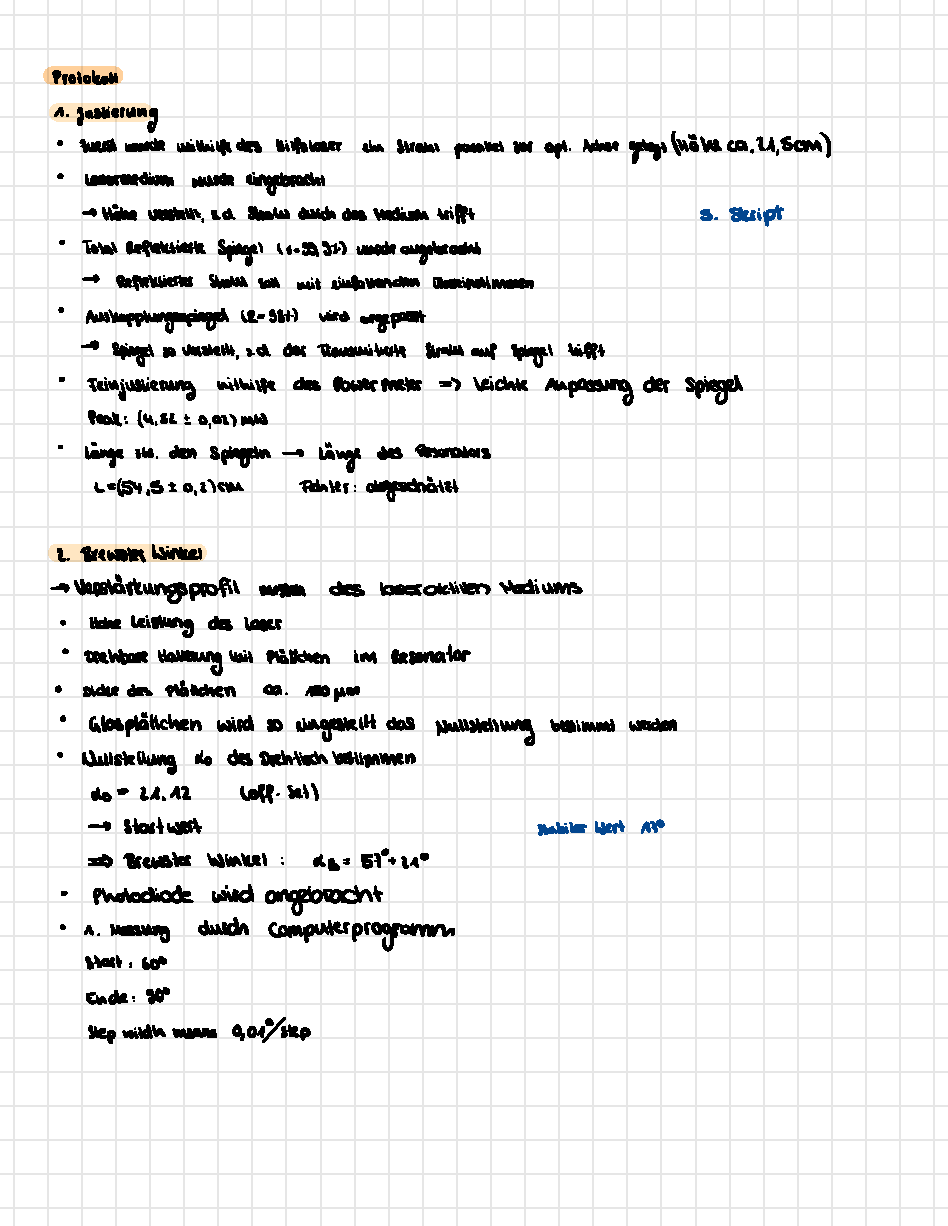
\includepdf[pages=1,landscape = false, offset=0 -25mm, scale=0.71,pagecommand ={\thispagestyle{empty}}\chapter{Protocol}]{Protokoll_Messung/Protokoll.pdf}

\includepdf[pages={2-4},scale=0.8,pagecommand ={\thispagestyle{plain}}]{Protokoll_Messung/Protokoll.pdf}
\chapter{Fehlerfortpflanzungen}
\section{Axiale Moden}
\textbf{Modenumrechnung:}
\begin{align}
    \nu&=\frac{x}{5,74\cdot10^{-3}\,\text{s}}\cdot\left(2\,\text{GHz}\right)\\
    s_\nu&=2,\text{GHz}\cdot\sqrt{\left(\frac{s_x}{5,74\cdot10^{-3}}\right)^2+\left(\frac{x}{\left(5,74\cdot10^{-3}\,\text{s}\right)^2}\cdot0,001\,\text{s}\right)^2}
\end{align}

\textbf{Auflösevermögen:}
\begin{align}
    A&=\frac{c}{\lambda\cdot\Delta\nu_m}\\
    s_A&=\left|s_{\Delta\nu_m}\frac{c}{\lambda\cdot\left(\Delta\nu_m\right)^2}\right|
\end{align}

\textbf{Finesse:}
\begin{align}
    F&=\frac{FSR}{\Delta\nu_m}\\
    F&=\left|s_{\Delta\nu_m}\frac{FSR}{\left(\Delta\nu_m\right)^2}\right|
\end{align}
\section{Bestimmung des Verstärkungsfaktor des laseraktiven Mediums}
\subsection{Messung der Intensität}
\textbf{Brechungsindex:}
\begin{align}
    n&=\tan\left(\alpha_B\right)\\
    s_n&=s_{\alpha_B}\cdot\frac{1}{\cos^2(\alpha_B)}
\end{align}
\subsection{Gewinn-Verlust-Bilanz}
\textbf{Verstärkung:}
\begin{align}
    \nu&=\frac{\ln\left(\frac{1}{R_1R_2T^2}\right)}{2\cdot l_\text{Medium}}\\
    s_\nu&=s_T\cdot\frac{1}{l_\text{Medium}\cdot T}
\end{align}

\textbf{Transmissionskoeffizient:}
\begin{align}
    T&=\left(\frac{1-R}{1+R}\right)^2\\
    s_T&=\left|s_R\cdot\frac{4\left(R-1\right)}{\left(R+1\right)^3}\right|
\end{align}

\textbf{Reflexionsgrad:}
\begin{align}
    R&=\frac{\tan^2\left(\alpha-\beta\right)}{\tan^2\left(\alpha+\beta\right)}\\
    s_R&=\frac{2\cdot\tan(\alpha-\beta)}{\tan^3\left(\alpha+\beta\right)}\sqrt{\left(s_\alpha\cdot\left(\frac{\tan(\alpha+\beta)}{\cos^2(\alpha-\beta)}+\frac{\tan(\alpha-\beta)}{\cos^2(\alpha+\beta)}\right)\right)^2+\left(s_\beta\cdot\left(\frac{\tan(\alpha+\beta)}{\cos^2(\beta-\alpha)}+\frac{\tan(\beta-\alpha)}{\cos^2(\alpha+\beta)}\right)\right)^2}
\end{align}

\textbf{Beta:}
\begin{align}
    \beta&=\frac{\arcsin(\alpha)}{n}\\
    s_\beta&=\sqrt{\left(s_n\cdot\frac{\arcsin(\alpha)}{n^2}\right)^2+\left(s_\alpha\cdot\frac{1}{\sqrt{1-\alpha^2}\cdot n}\right)^2}
\end{align}

\section{Gauß'sche Strahlenoptik}
\textbf{Brennweite der Linse:}
\begin{align}
    f&=\frac{s^2+z_R^2+2ss'\pm\sqrt{s^4+z_R^4+2s^2z_R^2-4(s')^2z_R^2}}{2(s'+s)}\\
    s_f&=\sqrt{\left(s_s\cdot\frac{\partial f}{\partial s}\right)^2+\left(s_s'\cdot\frac{\partial f}{\partial s'}\right)^2+\left(s_{z_R}\cdot\frac{\partial f}{\partial z_R}\right)^2}\\
    \frac{\partial f}{\partial s}&=\frac{-\frac{s^3+z_R^2s}{\sqrt{s^4+z_R^4+2s^2z_R^2-4(s')^2z_R^2}}+s+s'}{(s+s')}-\frac{s^2+2s's+z_R^2-\sqrt{s^4+z_R^4+2s^2z_R^2-4(s')^2z_R^2}}{2(s+s')^2}\\
    \frac{\partial f}{\partial s'}&=\frac{\frac{4z_R^2s'}{\sqrt{s^4+z_R^4+2s^2z_R^2-4(s')^2z_R^2}}+2s}{2(s+s')}-\frac{s^2+2s's+z_R^2-\sqrt{s^4+z_R^4+2s^2z_R^2-4(s')^2z_R^2}}{2(s+s')^2}\\
    \frac{\partial f}{\partial z_R}&=\frac{z_R}{s+s'}-\frac{z_R^3+4s^2z_R-4(s')^2z_R}{\left(s+s'\right)\cdot\sqrt{s^4+z_R^4+2s^2z_R^2-4(s')^2z_R^2}}\\
    z_R&=\frac{\pi w_0^2}{\lambda}\\
    s_{z_R}&=s_{w_0}\cdot\frac{2\pi w_0}{\lambda}
\end{align}

\textbf{Strahltaille im Resonator:}
\begin{align}
    w_{00}&=\sqrt{\frac{\lambda}{2\pi}\cdot\sqrt{L(2R-L)}}\\
    s_{w_{00}}&=s_L\cdot\sqrt{\frac{\lambda}{2\pi}}\cdot\frac{R-L}{((2R-L)L)^{\frac{3}{4}}}
\end{align}

\textbf{Theoretische Strahltaille:}
\begin{align}
    w_0&=\left(\frac{1}{w_{00}^2}\left(1-\frac{s}{f}\right)^2+\frac{1}{f^2}\left(\frac{\pi\cdot w_{00}}{\lambda}\right)^2\right)^{-\frac{1}{2}}\\
    s_{w_0}&=\sqrt{\left(s_{w_{00}}\cdot\frac{\partial w_0}{\partial w_{00}}\right)^2+\left(s_{f}\cdot\frac{\partial w_0}{\partial f}\right)^2+\left(s_{s}\cdot\frac{\partial w_0}{\partial s}\right)^2}\\
    \frac{\partial w_0}{\partial w_{00}}&=\frac{\frac{\pi^2w_{00}}{f^2\lambda^2}-\frac{\left(1-\frac{s}{f}\right)^2}{w_{00}^3}}{\left(\frac{\pi^2w_{00}^2}{f^2\lambda^2}+\frac{\left(1-\frac{s}{f}\right)^2}{w_{00}^2}\right)^{\frac{3}{2}}}\\
    \frac{\partial w_0}{\partial f}&=\frac{\frac{s-\frac{s^2}{f}}{f^2w_{00}^2}-\frac{\pi^2w_{00}^2}{\lambda^2f^3}}{\left(\frac{\pi^2w_{00}^2}{f^2\lambda^2}+\frac{\left(1-\frac{s}{f}\right)^2}{w_{00}^2}\right)^{\frac{3}{2}}}\\
    \frac{\partial w_0}{\partial s}&=\frac{1-\frac{s}{f}}{fw_{00}^2\left(\frac{\pi^2w_{00}^2}{f^2\lambda^2}+\frac{\left(1-\frac{s}{f}\right)^2}{w_{00}^2}\right)^{\frac{3}{2}}}
\end{align}

\textbf{Laserleistungsdichte:}
\begin{align}
    \frac{P}{A}&=\frac{(1-\frac{1}{e^2})\cdot P_{max}}{w_0^2\pi}\\
    s_{\frac{P}{A}}&=\sqrt{\left(s_{w_0}\cdot\frac{(1-\frac{1}{e^2})\cdot P_{max}}{2w_0^3\pi}\right)^2+\left(s_{P_{max}}\cdot\frac{(1-\frac{1}{e^2})}{w_0^2\pi}\right)^2}
\end{align}

%Literatur
\cleardoublepage
\bibliography{Literatur/Literatur}
\bibliographystyle{Literatur/LAuswertung}

%\newpage
%\listoffigures

\end{document}
%
% ------------------------------ Ende des Dokumentes -----------------------------------------
